\chapter{Teil 2: Klassifikation}
\label{chap:classification}
\section{Einleitung}\label{sec:classification}
Um eine Klassifizierung durchführen zu können, sind mehrere Komponenten notwendig, welche miteinander arbeiten. 
Dieser Ablauf wird in der \cref{fig:ablauf_klassifizierung} gezeigt.
\begin{figure}[H]
	\centering	
	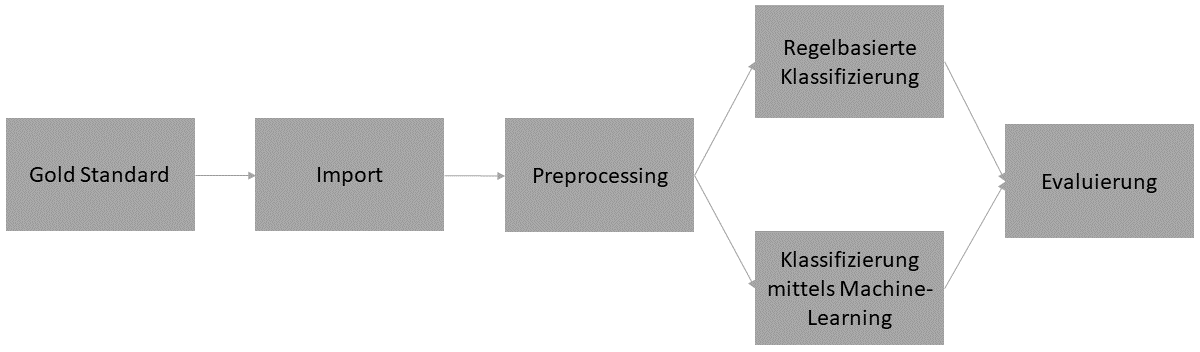
\includegraphics[width=1\columnwidth,keepaspectratio]{img/Ablauf_Klassifizierung.png}
	\caption{Pipeline}
	\source{Eigene Darstellung}
	\label{fig:ablauf_klassifizierung}
\end{figure}
Als Grundlage dienen die Daten des Gold Standards.
Diese werden mittels einer Import-Komponente geladen.
Bevor die Daten mit den entsprechenden Methoden klassifiziert werden, werden sie bei Bedarf noch vorverarbeitet.
Dann findet die eigentliche Klassifizierung statt.
Um eine möglichst präzise und erfolgreiche Variante des Klassifizierens zu finden, werden in diesem Teil der Arbeit mehrere Experimente durchgeführt.
Zum Schluss folgt eine Komponente, welche für das Auswerten der Klassifizierung und Ausgeben der Ergebnisse verantwortlich ist.
Bei dieser Klassifikation wird nicht zwischen den Kategorien \glqq Menüseite\grqq{} und \glqq Zeitlich ändernde Menüseite\grqq{} des Gold Standards unterschieden.
Diese Kategorien wurden zu einer Kategorie \glqq Menüseite\grqq{} zusammengeführt.
\section{Verwendete Technologien}
Folgend werden Technologien aufgelistet, welche einen hohen Stellenwert bei der Durchführung der Experimente eingenommen haben.
\subsection{Luigi}
Luigi ist ein Pipelining-Tool, welches vom Musikstreamingdienst Spotify entwickelt und später als Open-Source Projekt veröffentlicht worden ist\footnote{\url{https://github.com/spotify/luigi} abgerufen am 25.03.2019}.
Pipelining dient dazu, mehrere Tasks miteinander zu verknüpfen, das Ausführen zu Automatisieren und somit eine grössere Aufgabe zu verrichten.
Pipelining wird meist im Kontext von Big Data oder Machine-Learning angewendet, wo sich viele einzelne Tasks mit grossen Datenmengen beschäftigen.
Luigi wird selbst von Spotify selbst in der produktiven Umgebung verwendet und bietet unter anderem folgende Features:
\begin{itemize}
	\item Einzelne Tasks idempotent ausführen
	\item Teilschritte oder gesamte Pipeline kann über Konsolenausgabe oder Webinterface überwacht werden
	\item Fehlerfälle können protokolliert und dementsprechend reagiert werden
	\item Abhängigkeiten von Tasks werden selbstständig von Luigi gelöst
	\item Luigi ist komplett in Python aufgebaut und kann auch mit Python konfiguriert werden
\end{itemize}
Die einzelnen Tasks werden mit Python-Klassen realisiert.
Luigi ist so aufgebaut, dass jeder Task ein Input-File liest, von dem die Ausgabe des vorherigen Tasks eingelesen wird und ein Output-File schreibt, welches als Input-File des anschliessenden Tasks benutzt wird.
Dadurch kann Luigi die Zustände der einzelnen Tasks überwachen und im Falle eines Fehlers die Pipeline dort wieder starten, wo sie abgebrochen wurde.
Damit Luigi die Abhängigkeiten und das Überwachen bewerkstelligen kann, benötigt jede Klasse in der Pipeline folgende drei Funktionen:
\begin{itemize}
	\item Funktion requires() - Angabe auf welche Tasks Abhängigkeiten bestehen
	\item Funktion run() - Bereich, wo die eigentliche Logik des Tasks ist
	\item Funktion output() - Angabe, wohin die Ausgabe geschrieben wird
\end{itemize}
In dieser Arbeit wurde Luigi verwendet, um die einzelnen Tasks der Klassifizierung zu verknüpfen.

Es wurden zwei verschiedene Arten von Pipelines erstellt.
Die Entwicklungspipeline diente zur Entwicklung der Regeln/Machine-Learning-Modelle für die Klassifizierung.
Die Pipeline beinhaltet das Lesen der gecrawlten Daten, das Preprocessing, das Klassifizieren und das Evaluieren der Klassifizierung.
Sie beinhaltet folgende Komponenten:
\begin{itemize}
	\item Importer - Importiert die gecrawlten Websites und speichert sie in einer CSV-Datei
	\item Preprocessor - Wendet Preprocessing-Schritte an den Daten an
	\item RuleBasedClassifier - Regelbasierte Klassifizierung der Daten 
	\item MLClassifier - Klassifizierung der Daten mittels Machine-Learning
	\item Evaluator - Auswertung der Klassifizierung von Daten (nur im Entwicklunsmodus)
\end{itemize}
Die Produktionspipeline diente zur schlussendlichen Klassifizierung der Rohdaten anhand eines in der Entwicklungspipeline evaluierten Algorithmus.
\subsection{Scikit Learn}
Scikit Learn ist eine freie Programmierbibliothek für Python, mit welcher effizient Projekte für Data-Mining, Datenvisualisierung und Machine-Learning erarbeiten kann.
Scikit Learn ist unter BSD lizenziert und für die kommerzielle Nutzung frei verfügbar.
Sie ist eine der bekanntesten Standardbibliotheken für Machine-Learning, wird unter anderem von grossen Namen wie Google finanziell unterstützt und besitzt eine rege Contribution-Community auf Github\footnote{\url{https://github.com/scikit-learn/scikit-learn} abgerufen am: 07.05.2019}.\\
Scikit Learns Stärken liegen in den Machine-Learning Bereichen \glqq Supervised Learning\grqq{} und \glqq Unsupervised Learning\grqq{}.
Die API von Scikit Learn bietet eine Vielzahl von Algorithmen für Klassifizierung, Regression, Clustering, Dimensionsreduktion, Modelselektion sowie Preprocessing an und deckt somit die ganze Machine-Learning Pipeline ab\footnote{\url{https://scikit-learn.org/stable/} abgerufen am: 07.05.2019}.
Scikit Learn bietet für fast jeden Algorithmus oder Technik in der API eine Beispielimplementation an, welche für Fast-Prototyping  als Fundament übernommen werden kann.
\section{Preprocessing}
Das Preprocessing wurde entwickelt, um den Inhalt des Dokuments in eine standardisierte Form zu bringen.
Die folgenden Methoden können sowohl auf den Text eines Dokuments sowie auch auf den Titel angewendet werden.
Sie können mittels Konfiguration sowohl für den Text als auch Titel eines Dokuments ein- oder ausgeschaltet werden.
Der Link zum entsprechenden Code ist im \cref{app:classification} zu finden.
\subsection{Basis Preprocessing}
Um Text besser klassifizieren zu können, muss dieser zuerst bereinigt und standardisiert werden\footnote{\url{https://machinelearningmastery.com/clean-text-machine-learning-python/} abgerufen am: 11.07.2019}.
Die nachfolgenden Methoden des Basis Preprocessing werden in jedem Fall der Klassifikation durchgeführt.
Sie verändern jeweils nur einzelne Zeichen des Textes.
\subsubsection{Gross-/Kleinschreibung}
Alle Buchstaben, welche grossgeschrieben sind, werden durch die entsprechenden Kleinbuchstaben ersetzt.
\subsubsection{Umlaute ersetzen}
Umlaute werden durch ihre verwandten Selbstlaute ersetzt, genauer:
\begin{itemize}
	\item ä $\rightarrow$ a
	\item ö $\rightarrow$ o
	\item ü $\rightarrow$ u
\end{itemize} 
\subsubsection{Sonderzeichen entfernen}
Alle Sonderzeichen, die nicht in der folgenden Auflistung vorkommen, werden durch einen Leerschlag ersetzt:
\begin{itemize}
	\item éàèÉÀÈäöüÄÖÜa-zA-Z
\end{itemize} 
\subsubsection{Einzelne Zeichen entfernen}
Jedes einzelne Zeichen, also solche, die sowohl vorne als auch hinten an einen Leerschlag angrenzen, werden entfernt.
\subsubsection{Multiple Leerschläge entfernen}
Da durch die vorhergehenden Schritte oft multiple Leerschläge anfallen, werden diese auf einen Leerschlag reduziert.
\subsection{Fortgeschrittenes Preprocessing}\label{sec:advancedpre}
Die nachfolgenden Methoden stellen das fortgeschrittene Preprocessing dar.
Im Gegensatz zum Basis Preprocessing ersetzen, löschen oder verändern sie ganze Wörter im Text.
\subsubsection{Preisdetektor}
Da Menüs häufig in Verbindung mit Preisen vorkommen und in weiteren Preprocessing-Schritten Zahlen und Sonderzeichen entfernt werden, ist es von Vorteil, diese Informationen nicht zu verlieren.
Daher erkennt diese Methode verschiedene Varianten von Preisen mittels regulären Ausdrücken (Regex, Regular Expression) und ersetzt diese mit einem Schlüsselwort.
% Varianten genauer ausführen
Die folgenden Varianten von Preisen wird erkannt:
\begin{itemize}
	\item Preisangabe + chf/fr/sfr
	\item Preisangabe
	\item chf/fr/sfr + Preisangabe
\end{itemize} 
Zudem wird unterschieden, wie viele Stellen der Preis hat.
Die nun aufgeführte Liste zeigt die verschiedenen Schlüsselwörter:
\begin{itemize}
	\item Einstellig $\rightarrow$ onedigitprice
	\item Zweistellig $\rightarrow$ twodigitprice
	\item Dreistellig $\rightarrow$ threedigitprice
\end{itemize} 
Um Zeitangaben nicht als Preise zu erkennen, werden bei Preisangaben ohne Währungsangabe nur Beträge mit Rappenbeträgen, welche 60 oder höher sind, erkannt.
\subsubsection{Stammformreduktion}
Dieses Verfahren führt verschiedene morphologische Varianten eines Wortes auf ihren gemeinsamen Stamm zurück.
Dafür wird der Stemmer \glqq Cistem\footnote{\url{https://github.com/LeonieWeissweiler/CISTEM} abgerufen am: 18.03.2019}\grqq{} verwendet, da für die deutsche Sprache nur wenig Alternativen vorhanden sind.
Ein Beispiel: Die Wörter \glqq Preise\grqq{} und \glqq Preisen\grqq{} werden beide auf \glqq Preis\grqq{} reduziert.
\subsubsection{Getränkedetektor}
% Referenz Cistem
Eine Liste mit Einträgen diverser Getränke bildet die Grundlage dieser Methode.
Wenn im Text ein Getränk dieser Liste vorhanden ist, wird es durch das Schlüsselwort \glqq beverageentity\grqq{} ersetzt.
Damit soll erreicht werden, dass ein einheitliches Merkmal geschaffen wird.
\subsubsection{Stoppwörter entfernen}
Bei Stoppwörter handelt es sich um Wörter, welche keine Relevanz für den Inhalt eines Texts haben, aber oft vorkommen, wie z.B. \glqq in\grqq{}, \glqq auf\grqq{} und \glqq oder\grqq{}.
Eine Stoppwortliste führt 1720 solcher Wörter in Deutsch auf. Sie ist aus mehreren Quellen zusammengesetzt worden.
Wenn eines dieser Wörter im Text vorkommt, wird es entfernt.
\section{Regelbasierte Experimente}
Die folgenden Experimente beschreiben die Methoden und Resultate der regelbasierten Experimente.
Anschliessend folgt die Interpretation und Diskussion.
Der Link zum entsprechenden Code ist im Anhang (\cref{app:classification}) zu finden.
\subsection{Regelsatz: Menü im Titel}
\subsubsection{Methode}
Dieser simple Algorithmus überprüft, ob der Begriff \glqq menu\grqq{} in einem Wort des Metatags \glqq Title\grqq{} vorkommt.
Falls ja, wird das Dokument als Menüseite klassiert.
\subsubsection{Resultate}
Für dieses Regelset sind keine Parameter verfügbar, daher ist nur eine Konfiguration durchgeführt worden.
Diese hat anhand der Trainingsdaten folgende Metriken ergeben:\\
\begin{table}[H]
	\centering
	\begin{tabular}{|l|l|l|}
		\hline
		F1-Score & Precision & Recall\\
		\hline
		0.17 & 0.43 & 0.11  \\
		\hline
	\end{tabular}
	\caption{Score des Regelsets: Menü im Titel anhand der Trainingsdaten}
	\source{Eigene Darstellung}
\end{table}
Das folgende Ergebnis ist anhand der Daten des Testsets entstanden:
\begin{table}[H]
	
	\centering
	\begin{tabular}{|l|l|l|l|}
		\hline
		Methode & F1-Score & Precision & Recall\\
		\hline
		Menü im Titel & 0.28 & 1.00 & 0.16 \\
		\hline
	\end{tabular}
	\caption{Score des Regelsatzes: Menü im Titel anhand der Testdaten}
	\source{Eigene Darstellung}
\end{table}
Die Klassifizierung in absoluten Zahlen wird mittels Konfusionsmatrix verdeutlicht.
\begin{table}[H]
	\centering
	\begin{tabular}{@{}cc|cc@{}}
		\multicolumn{1}{c}{} &\multicolumn{1}{c}{} &\multicolumn{2}{c}{Predicted} \\ 
		\multicolumn{1}{c}{} & 
		\multicolumn{1}{c|}{} & 
		\multicolumn{1}{c}{Positiv} & 
		\multicolumn{1}{c}{Negativ} \\ 
		\cline{2-4}
		\multirow[c]{2}{*}{\rotatebox[origin=tr]{90}{Actual}}
		& Positiv  & 8   & 42   \\[1.5ex]
		& Negativ  & 0   & 50 \\ 
		\cline{2-4}
	\end{tabular}
	\caption{Konfusionsmatrix des Regelsets: Menü im Titel anhand der Testdaten}
	\source{Eigene Darstellung}
\end{table}
\subsection{Regelsatz: Preisdetektor}
\subsubsection{Methode}
Dieser Algorithmus funktioniert dank der Preprocessing-Methode, welche den Preis erkennt und mit einem Schlüsselwort ersetzt.
Sofern dieses Schlüsselwort für zweistellige Preise im Text vorhanden ist, wird das Dokument als Menüseite klassifiziert. 
Dies unter der Annahme, dass Menüpreise oft zweistellig, im Gegensatz zu Getränkepreisen welche häufig einstellig und Hotelpreisen, die meist dreistellig sind.
Die Anzahl vorhandener Preise kann über die Konfiguration angegeben werden.
\subsubsection{Resultate}
Durch die Konfiguration kann ein Schwellwert für die Anzahl erkannter Preise angegeben werden, die vorhanden sein müssen, um eine Webpage als positiv zu klassifizieren.\\
\begin{table}[H]
	\centering
	\begin{tabular}{|l|l|l|l|}
		\hline
		Schwellwert & F1-Score & Precision & Recall\\
		\hline
		1 & 0.45 & 0.36 & 0.60  \\
		2 & 0.46 & 0.45 & 0.47 \\
		3 & 0.41 & 0.49 & 0.36 \\
		\hline
	\end{tabular}
	\caption{Scores des Regelsets: Preisdetektor anhand der Trainingsdaten}
	\source{Eigene Darstellung}
\end{table}
Das beste Ergebnis hat ein Schwellwert von zwei erzielt, danach ist der F1-Score wieder schlechter geworden.
Daraus wurde geschlussfolgert, dass für dieses Regelset das Maximum bereits erreicht wurde.
\\
Das folgende Ergebnis ist anhand der Daten des Testsets entstanden:
\begin{table}[H]
	\centering
	\begin{tabular}{|l|l|l|l|}
		\hline
		Methode & F1-Score & Precision & Recall\\
		\hline
		Preisdetektor & 0.65 & 0.93 & 0.50 \\
		\hline
	\end{tabular}
	\caption{Score des Regelsatzes: Preisdetektor anhand der Testdaten} 
	\source{Eigene Darstellung}
\end{table}
Die Klassifizierung in absoluten Zahlen wird mittels Konfusionsmatrix verdeutlicht.
\begin{table}[H]

	\centering
	\begin{tabular}{@{}cc|cc@{}}
		\multicolumn{1}{c}{} &\multicolumn{1}{c}{} &\multicolumn{2}{c}{Predicted} \\ 
		\multicolumn{1}{c}{} & 
		\multicolumn{1}{c|}{} & 
		\multicolumn{1}{c}{Positiv} & 
		\multicolumn{1}{c}{Negativ} \\ 
		\cline{2-4}
		\multirow[c]{2}{*}{\rotatebox[origin=tr]{90}{Actual}}
		& Positiv  & 25   & 25   \\[1.5ex]
		& Negativ  & 2    & 48 \\ 
		\cline{2-4}
	\end{tabular}
	\caption{Konfusionsmatrix des Regelsets: Preisdetektor anhand der Testdaten}
	\source{Eigene Darstellung}
\end{table}
\subsection{Regelsatz: Kombination aus Menü im Titel und Preisdetektor}
\subsubsection{Methode}
Diese Kombination führt eine sequenzielle Klassifikation aus.
Im ersten Schritt wird der Mechanismus des Algorithmus \glqq Menü im Titel\grqq{} verwendet.
Falls durch diesen keine positive Klassifikation zustande kommt, wird durch den Preisdetektor nochmals neu klassifiziert.
\subsubsection{Resultate}
Bei dieser Konfiguration kann der Schwellwert ebenfalls für die Anzahl erkannter Preise angegeben werden.\\
\begin{table}[H]
	\centering
	\begin{tabular}{|l|l|l|l|}
		\hline
		Schwellwert & F1-Score & Precision & Recall\\
		\hline
		1 & 0.45 & 0.35 & 0.65 \\
		2 & 0.47 & 0.43 & 0.52 \\
		3 & 0.43 & 0.45 & 0.41 \\
		\hline
	\end{tabular}
	\caption{Scores des Regelsets: Kombination aus Menü im Titel und Preisdetektor anhand der Trainingsdaten}
	\source{Eigene Darstellung}
\end{table}
Auch bei diesem Regelset hat die Konfiguration mit einem Schwellwert von zwei das beste Ergebnis erzielt.
\\
Das folgende Ergebnis ist anhand der Daten des Testsets entstanden:
\begin{table}[H]
	\centering
	\begin{tabular}{|l|l|l|l|}
		\hline
		Methode & F1-Score & Precision & Recall\\
		\hline
		Kombination aus Menü im Titel und Preisdetektor & 0.70 & 0.93 & 0.56\\
		\hline
	\end{tabular}
	\caption{Score des Regelsatzes: Kombination aus Menü im Titel und Preisdetektor anhand der Testdaten}
	\source{Eigene Darstellung}
\end{table}
Die Klassifizierung in absoluten Zahlen wird mittels Konfusionsmatrix verdeutlicht.
\begin{table}[H]
	\centering
	\begin{tabular}{@{}cc|cc@{}}
		\multicolumn{1}{c}{} &\multicolumn{1}{c}{} &\multicolumn{2}{c}{Predicted} \\ 
		\multicolumn{1}{c}{} & 
		\multicolumn{1}{c|}{} & 
		\multicolumn{1}{c}{Positiv} & 
		\multicolumn{1}{c}{Negativ} \\ 
		\cline{2-4}
		\multirow[c]{2}{*}{\rotatebox[origin=tr]{90}{Actual}}
		& Positiv  & 28   & 22   \\[1.5ex]
		& Negativ  & 2   & 48 \\ 
		\cline{2-4}
	\end{tabular}
	\caption{Konfusionsmatrix des Regelsets: Kombination aus Menü im Titel und Preisdetektor anhand der Testdaten}
	\source{Eigene Darstellung}
\end{table}
\subsection{Regelsatz: Listing}
\subsubsection{Methode}
Dieser Algorithmus basiert sowohl auf dem Blacklisting- als auch auf dem Whitelisting-Ansatz.
Dazu wird eine Blacklist und eine Whitelist verwendet, die von Hand erstellt wurden und Einträge enthalten, welche für die jeweiligen Kategorien typisch sind.
Falls ein Wort aus der Black- oder Whitelist im Text einer Webpage vorkommt, wird ein entsprechender Zähler hochgezählt.
Zum Schluss findet eine sequenzielle Klassifizierung statt, das heisst: 
Wenn der Zähler der Blacklist einen konfigurierbaren Schwellwert überschreitet, wird die Webpage als negativ klassifiziert. 
Wenn der Zähler der Whitelist einen konfigurierbaren Schwellwert überschreitet, wird die Webpage als Menüseite klassifiziert.
Falls kein Zähler oder beide den Schwellwert überschreitet, wird die Webpage ebenfalls als negativ klassifiziert. 
\subsubsection{Resultate}
In einem ersten Versuch wurden identische Schwellwerte gewählt und jeweils erhöht:\\
\begin{table}[H]
	\centering
	\begin{tabular}{|l|l|l|l|l|}
		\hline
		Schwellwert Whitelist & Schwellwert Blacklist & F1-Score & Precision & Recall\\
		\hline
		1 & 1 & 0.17 & 0.32 & 0.11 \\
		5 & 5 & 0.39 & 0.62 & 0.29 \\
		10 & 10 & 0.42 & 0.77 & 0.29 \\
		20 & 20 & 0.33 & 0.85 & 0.21 \\
		30 & 30 & 0.27 & 0.91 & 0.16 \\
		\hline
	\end{tabular}
	\caption{Scores der ersten Iteration des Regelsets: Listing anhand der Trainingsdaten}
	\source{Eigene Darstellung}
\end{table}
Dieser Versuch hat gezeigt, dass ein maximaler F1-Score bei gleichen Werten zwischen 5 und 20 zu erreichen ist.\\
Da gleich gewählte Werte keine zufriedenstellende Ergebnisse erzielten, wurden im zweiten Versuch unterschiedliche Verhältnisse getestet:\\
\begin{table}[H]
	\centering
	\begin{tabular}{|l|l|l|l|l|}
		\hline
		Schwellwert Whitelist & Schwellwert Blacklist & F1-Score & Precision & Recall\\
		\hline
		5 & 1 & 0.12 & 0.82 & 0.07 \\
		1 & 5 & 0.31 & 0.24 & 0.45 \\
		\hline
	\end{tabular}
	\caption{Scores der zweiten Iteration des Regelsets: Listing anhand der Trainingsdaten}
	\source{Eigene Darstellung}
\end{table}
Aus diesem Versuch entstand die Erkenntnis, dass ein höherer Schwellwert der Blacklist als der Whitelist erforderlich ist, um einen möglichst hohen Score zu erreichen.
Diese Erkenntnis wurde in einem weiteren Versuch in mehreren Iterationen getestet:\\
\begin{table}[H]
	\centering
	\begin{tabular}{|l|l|l|l|l|}
		\hline
		Schwellwert Whitelist & Schwellwert Blacklist & F1-Score & Precision & Recall\\
		\hline
		2 & 10 & 0.42 & 0.33 & 0.61 \\
		3 & 15 & 0.52 & 0.42 & 0.70 \\
		3 & 20 & 0.51 & 0.39 & 0.75 \\
		4 & 15 & 0.53 & 0.47 & 0.61 \\
		5 & 15 & 0.55 & 0.54 & 0.56 \\
		5 & 20 & 0.54 & 0.50 & 0.60 \\
		5 & 21 & 0.54 & 0.49 & 0.60 \\
		6 & 20 & 0.55 & 0.56 & 0.55 \\
		7 & 20 & 0.55 & 0.60 & 0.50 \\
		8 & 20 & 0.53 & 0.64 & 0.46 \\
		\hline
	\end{tabular}
	\caption{Scores der dritten Iteration des Regelsets: Listing anhand der Trainingsdaten}
	\source{Eigene Darstellung}
\end{table}
Die Schwellwerte wurden stetig erhöht.
Dabei wurden verschiedene Schwellwerte in unterschiedlichen Verhältnissen getestet.
Sobald einer dieser Schwellwerte zu einem schlechteren Ergebnis geführt hat, wurde er wieder reduziert oder ein neues Verhältnis getestet.
Beim Verhältnis 6/20 bzw. 7/20 wurde das Maximum des F1-Scores erreicht.
Da diese Werte nicht im Bereich einer zufriedenstellenden Klassifikation sind, wurde auf die Ermittlung aller möglichen Kombinationen verzichtet.
\\
Das folgende Ergebnis ist anhand der Daten des Testsets entstanden:
\begin{table}[H]
	\centering
	\begin{tabular}{|l|l|l|l|}
		\hline
		Methode & F1-Score & Precision & Recall\\
		\hline
		Listing & 0.68 & 0.96 & 0.52\\
		\hline
	\end{tabular}
	\caption{Score des Regelsatzes: Listing anhand der Testdaten}
	\source{Eigene Darstellung}
\end{table}
Die Klassifizierung in absoluten Zahlen wird mittels Konfusionsmatrix verdeutlicht.
\begin{table}[H]
	\centering
	\begin{tabular}{@{}cc|cc@{}}
		\multicolumn{1}{c}{} &\multicolumn{1}{c}{} &\multicolumn{2}{c}{Predicted} \\ 
		\multicolumn{1}{c}{} & 
		\multicolumn{1}{c|}{} & 
		\multicolumn{1}{c}{Positiv} & 
		\multicolumn{1}{c}{Negativ} \\ 
		\cline{2-4}
		\multirow[c]{2}{*}{\rotatebox[origin=tr]{90}{Actual}}
		& Positiv  & 26   & 24   \\[1.5ex]
		& Negativ  & 1    & 49 \\ 
		\cline{2-4}
	\end{tabular}
	\caption{Konfusionsmatrix des Regelsets: Listing anhand der Testdaten}
	\source{Eigene Darstellung}
\end{table}
\subsection{Regelsatz: Bag of Words}
\subsubsection{Methode}
Dieser Algorithmus basiert auf der statistischen Methode \glqq Bag of Words\grqq{}.
Bag of Words zählt für jedes Dokument der Trainingsdaten, wie oft ein Wort darin vorkommt.
In dieser Anwendung wird jedoch nur erkannt, ob ein Wort vorkommt, oder nicht, die Anzahl spielt keine Rolle (binäres Bag of Words).
Anhand dieser Wörter wird eine dynamische Black- und Whitelist erstellt, Wörter die in beiden Listen vorkommen, werden entfernt.
Dafür wird der komplette Trainingsdatensatz des Gold Standards in einen Trainings- und Testsatz in einem konfigurierbaren Verhältnis aufgeteilt.
Anhand dieser Listen wird der Testdatensatz klassifiziert.
Die Anzahl der Wörter dieser Listen ist konfigurierbar.
Die Klassifikation findet mittels einem Zähler statt.
Für jedes Wort eines Dokuments, welches in der Liste der positiven Beispielen vorkommt, wird der Zähler hochgezählt, für jedes Wort aus der Liste der negativen Beispielen wird er heruntergezählt.
Für die Klassifizierung wird der Zähler mit einem konfigurierbaren Schwellwert verglichen, Falls der Zähler grösser ist als der Schwellwert, wird das Dokument als positiv klassifiziert, ansonsten negativ.
Um die Ergebnisse anhand der Testdaten evaluieren zu können, sind diese Listen (diejenigen der Konfiguration, welche auf den Trainingsdaten das beste Ergebnis lieferten) zudem persistent implementiert worden.
\subsubsection{Resultate}
Bei diesem Regelset kann die Grösse der Black- und Whitelist (Features), das Verhältnis zwischen Test- und Trainingsdaten (Split) sowie ein Schwellwert angegeben werden.
Für das Verhältnis zwischen Test- und Trainingsdaten wurden die Werte 0.3, 0.5 und 0.7 getestet.
In einer ersten Iteration wurde die Anzahl von 200 Features und ein Split von 0.3 verwendet, um herauszufinden, ob ein positiver oder negativer Schwellwert bessere Werte erzielt.\\
\begin{table}[H]
	\centering
	\begin{tabular}{|l|l|l|l|}
		\hline
		Schwellwert & F1-Score & Precision & Recall\\
		\hline
		0 & 0.64 & 0.58 & 0.71 \\
		2 & 0.51 & 0.38 & 0.75 \\
		-2 & 0.68 & 0.74 & 0.63 \\
		\hline
	\end{tabular}
	\caption{Scores der ersten Iteration des Regelsets: Bag of Words anhand der Trainingsdaten}
	\source{Eigene Darstellung}
\end{table}
Dabei wurde erkannt, dass sich ein negativer Schwellwert positiv auf den F1-Score auswirkt.\\
In der zweiten Iteration wurde der Schwellwert weiter verkleinert.\\
\begin{table}[H]
	\centering
	\begin{tabular}{|l|l|l|l|}
		\hline
		Schwellwert & F1-Score & Precision & Recall\\
		\hline
		-3 & 0.66 & 0.80 & 0.57 \\
		-4 & 0.66 & 0.86 & 0.54 \\
		-5 & 0.66 & 0.89 & 0.52 \\
		\hline
	\end{tabular}
	\caption{Scores der zweiten Iteration des Regelsets: Bag of Words anhand der Trainingsdaten}
	\source{Eigene Darstellung}
\end{table}
Da diese Werte sich fast nicht unterscheiden, wurden alle weiterverwendet, um einen maximalen Score zu evaluieren.
In einer dritten, ausführlicheren Iteration sind die Anzahl Features von 200 bis 400 sowie die drei oben genannten Verhältnisse zusammen mit den vier Schwellwerten getestet worden. Die \cref{tab:bow3} zeigt diese Tests, sortiert nach bestem F1-Score:\\
\FloatBarrier
\begin{table}
	\centering
	\label{tab:bow3}
	\begin{tabular}{ | l | l | l | l | l | l | }
		\hline
		Split & Features & Limit & F1-Score & Precision & Recall \\ \hline
		0.3 & 400 & -3 & 0.72 & 0.74 & 0.7 \\ 
		0.3 & 400 & -4 & 0.72 & 0.79 & 0.66 \\
		0.3 & 400 & -5 & 0.72 & 0.81 & 0.64 \\
		0.7 & 400 & -3 & 0.72 & 0.75 & 0.69 \\
		0.7 & 400 & -4 & 0.72 & 0.79 & 0.66 \\
		0.5 & 300 & -3 & 0.71 & 0.79 & 0.65 \\
		0.5 & 400 & -3 & 0.70 & 0.74 & 0.67 \\
		0.5 & 400 & -4 & 0.70 & 0.79 & 0.63 \\ 
		0.7 & 400 & -2 & 0.70 & 0.70 & 0.70 \\ 
		0.7 & 300 & -3 & 0.70 & 0.74 & 0.67 \\
		0.7 & 300 & -4 & 0.70 & 0.80 & 0.63 \\
		0.7 & 300 & -5 & 0.70 & 0.84 & 0.60 \\
		0.7 & 400 & -5 & 0.70 & 0.82 & 0.62 \\ 
		0.3 & 400 & -2 & 0.69 & 0.66 & 0.73 \\ 
		0.5 & 400 & -2 & 0.69 & 0.69 & 0.69 \\ 
		0.5 & 400 & -5 & 0.69 & 0.82 & 0.60 \\ 
		0.7 & 200 & -3 & 0.69 & 0.76 & 0.63 \\ 
		0.7 & 200 & -4 & 0.69 & 0.81 & 0.60 \\ 
		0.3 & 300 & -2 & 0.68 & 0.73 & 0.64 \\ 
		0.3 & 300 & -3 & 0.68 & 0.78 & 0.60 \\ 
		0.3 & 200 & -2 & 0.68 & 0.74 & 0.63 \\ 
		0.5 & 200 & -3 & 0.68 & 0.77 & 0.60 \\ 
		0.5 & 300 & -4 & 0.68 & 0.81 & 0.59 \\ 
		0.7 & 300 & -2 & 0.68 & 0.69 & 0.68 \\ 
		0.5 & 200 & -2 & 0.67 & 0.71 & 0.64 \\ 
		0.3 & 300 & -4 & 0.66 & 0.82 & 0.56 \\ 
		0.3 & 200 & -3 & 0.66 & 0.80 & 0.57 \\
		0.3 & 200 & -4 & 0.66 & 0.86 & 0.54 \\
		0.3 & 200 & -5 & 0.66 & 0.89 & 0.52 \\ 
		0.5 & 200 & -4 & 0.66 & 0.81 & 0.56 \\
		0.5 & 300 & -5 & 0.66 & 0.83 & 0.55 \\ 
		0.7 & 200 & -2 & 0.66 & 0.66 & 0.66 \\ 
		0.7 & 200 & -5 & 0.66 & 0.85 & 0.55 \\ 
		0.3 & 300 & -5 & 0.65 & 0.85 & 0.52 \\ 
		0.5 & 200 & -5 & 0.65 & 0.87 & 0.52 \\
		0.5 & 300 & -2 & 0.46 & 0.62 & 0.36 \\ \hline
	\end{tabular}
	\caption{Scores der dritten Iteration des Regelsets: Bag of Words anhand der Trainingsdaten}
	\source{Eigene Darstellung}
\end{table}
Daraus lässt sich schliessen, dass eine hohe Anzahl Features zu einem besseren Ergebnis führt.
Das Verhältnis zwischen Test- und Trainingsdaten ist nicht so relevant, da sowohl das Verhältnis 0.3 als auch 0.7 zu hohen Scores führt.
Der Schwellwert ist im Bereich -2 bis -5 ebenfalls nicht aussagekräftig, da auch dieser bei den besten Scores vertreten ist.
Es muss zudem berücksichtigt werden, dass der Split zufällig gewählt wird und keine Kreuzvalidierung stattfindet, dadurch können diese Ergebnisse variieren.
\FloatBarrier

Das folgende Ergebnis ist anhand der Daten des Testsets entstanden:
\begin{table}[H]
	\centering
	\begin{tabular}{|l|l|l|l|}
		\hline
		Methode & F1-Score & Precision & Recall\\
		\hline
		Bag of Words & 0.74 & 0.91 & 0.62\\
		\hline
	\end{tabular}
	\caption{Score des Regelsatzes: Bag of Words anhand der Testdaten}
	\source{Eigene Darstellung}
\end{table}
Die Klassifizierung in absoluten Zahlen wird mittels Konfusionsmatrix verdeutlicht.
\begin{table}[H]
	\centering
	\begin{tabular}{@{}cc|cc@{}}
		\multicolumn{1}{c}{} &\multicolumn{1}{c}{} &\multicolumn{2}{c}{Predicted} \\ 
		\multicolumn{1}{c}{} & 
		\multicolumn{1}{c|}{} & 
		\multicolumn{1}{c}{Positiv} & 
		\multicolumn{1}{c}{Negativ} \\ 
		\cline{2-4}
		\multirow[c]{2}{*}{\rotatebox[origin=tr]{90}{Actual}}
		& Positiv  & 31   & 19   \\[1.5ex]
		& Negativ  & 3    & 47 \\ 
		\cline{2-4}
	\end{tabular}
	\caption{Konfusionsmatrix des Regelsets: Bag of Words anhand der Testdaten}
	\source{Eigene Darstellung}
\end{table}
\section{Experimente mittels Machine-Learning}
\subsection{Einleitung}
\subsubsection{Durchführung der Experimente}
Alle Experimente werden mit der Pipeline, welche im \cref{sec:classification} beschrieben wird, durchgeführt.
Um eine möglichst grosse Abdeckung von Experimenten zu erzielen, werden bei jedem Experiment drei parallele Pipelines verwendet, die jeweils eine andere Feature-Extraction Methode verwenden.
Die drei verwendeten Feature-Extraction Methoden sind \glqq Bag of Words\grqq{}, \glqq binäres Bag of Words\grqq{} und \glqq TF-IDF\grqq{}, welche in \cref{sub:bow} und \cref{sub:tfidf} erläutert werden.\\
Für jede Pipeline wurde vor dem Training der Algorithmen, welche im \cref{sub:clf} ersichtlich sind, aus den Trainingsdaten eine kleine Teilmenge als Validierungsset entnommen.
Die einzelnen Pipelines wurden danach mit dem Rest des Trainingssets trainiert und mit dem entnommenen Validierungsset validiert.
Dies wurde konsequent für alle Experimente durchgeführt, um eine unverzerrte Einschätzung der Performance der Algorithmen während der Experimente zu erhalten.
Würde man die Validierung auf den Trainingsdaten durchführen, hätte man eine verzerrte Einschätzung der Performance\footnote{\url{https://machinelearningmastery.com/difference-test-validation-datasets/} abgerufen am: 10.07.2019}.\\
Zusätzlich wurde nach Abschluss aller Experimente die Performance des besten Klassifizierers auf einem ungesehenen Testdatenset überprüft.
Diese Überprüfung gibt einen Rückschluss darauf, wie gut der Klassifizierer auf ungesehene Daten generalisierte Einschätzungen geben kann.
\subsubsection{Konfigurationen zu den einzelnen Experimenten}
Jede ausgeführte Pipeline erzeugt eine Textdatei mit den Ergebnissen und der Konfiguration der Pipeline.
Somit kann jedes Ergebnis der Experimente wiederholt und nachvollzogen werden.
Alle Textdateien können im Anhang \cref{app:electronic} im Zip-Ordner mit den Log- und Konfigurationsdateien gefunden werden.
Es wird in diesem Kapitel verzichtet, jeweils die Konfigurationen aufzulisten, um den Lesefluss nicht zu stören.
Für genauere Einblicke in die einzelnen Konfigurationen kann der oben erwähnte Anhang miteinbezogen werden.\\
Als Einstiegspunkt für die Experimente wurde das erste Experiment mit einer Anzahl Features von 100, eingeschalteten Basis-Preprocessing-Methoden sowie der Standardkonfigurationen von Scikit-Learn für alle drei Feature-Extraction Methoden ausgeführt.\\
Alle Experimente wurden sequentiell durchgeführt und die Erkenntnisse des vorherigen Experiments in die Konfigurationen des nächsten Experiments miteinbezogen.
\subsubsection{Bag of Words und binäres Bag of Words}\label{sub:bow}
Der statistische Ansatz namens \glqq Bag of Words\grqq{} wandelt einen Text in eine Anhäufung von Wörtern um, ohne dabei die sequentielle Abhängigkeit der Wörter zu berücksichtigen.
Danach wird für jedes Wort die Häufigkeit des Vorkommens in dieser Anhäufung gezählt und hinterlegt.
Bag of Words erstellt im Grunde ein Histogramm aller Wörter eines Textes.
Ebenfalls kann die boolsche Häufigkeit (Term vorhanden/nicht vorhanden) verwendet werden, damit man nur ein Set von allen im Text vorkommenden Wörtern erhält.
\subsubsection{TF-IDF}\label{sub:tfidf}
TF-IDF (TermFrequency-InverseDocumentFrequency) ist eine Methodik zur Bestimmung der Relevanz eines Terms in einer Sammlung von Dokumenten (Dokumentkorpus).\\
TF-IDF wird aus den zwei folgenden Metriken zusammengesetzt.
\begin{itemize}
	\item TF
	\begin{itemize}
		\item Termfrequenz berechnet die Häufigkeit eines Terms in einem Dokument im Verhältnis zur gesamten Anzahl Terme. Dies erreicht eine Normalisierung der Termfrequenz, da bei langen Texten der Term potentiell öfters vorkommen kann.\\
	\end{itemize}
	\item IDF
	\begin{itemize}
		\item Inverse Dokumentfrequenz hingegen ermittelt nun die Relevanz der Terme, indem berechnet wird, wie viele Dokumente den Term T enthalten. Die gesamte Anzahl an Dokumenten wird durch die ermittelte Anzahl von Dokumenten mit Term T dividiert und mit dem natürlichen Logarithmus logarithmiert.\\
		Somit ist ein Term, welcher in vielen Dokumenten vorkommt, weniger relevant als ein rarer Term.
	\end{itemize}
	\item TF-IDF
	\begin{itemize}
		\item TF-IDF ist nun die Multiplikation von TF und IDF.
	\end{itemize}
\end{itemize}
TF-IDF stammt aus der Disziplin \glqq Information Retrieval\grqq{} und findet dank der Gewichtung von Wörtern im Machine-Learning Bereich hohen Anklang\footnote{\url{http://www.tfidf.com/} abgerufen am: 07.05.2019}.
\subsubsection{Übersicht der verwendeten Machine-Learning Algorithmen}\label{sub:clf}
Aufgrund des \glqq No free lunch\grqq{}-Theorems wurden 14 Algorithmen trainiert und validiert.
Nun erfolgt eine Auflistung aller Algorithmen, die verwendet wurden.
Zusätzlich können die Algorithmen im \cref{sec:algos} nachgeschlagen werden.
\begin{itemize}
	\item Lineare Modelle
	\begin{itemize}
		\item Ridge Classifier
		\item Perceptron
		\item PassiveAgressiveClassifier
		\item SGDClassifier (Stochastic Gradient Descent)
	\end{itemize}
	\item Naive Bayes Modelle
	\begin{itemize}
		\item Bernoulli-Naive-Bayes
		\item Complement-Naive-Bayes
		\item Multinomial-Naive-Bayes
		\item Gaussian-Naive-Bayes
	\end{itemize}
	\item Tree Modelle
	\begin{itemize}
		\item DecisionTreeClassifier
	\end{itemize}
	\item Ensemble Modelle
	\begin{itemize}
		\item RandomForestClassifier
		\item AdaBoostClassifier
	\end{itemize}
	\item Nearest Neighbor Modelle
	\begin{itemize}
		\item KNeighborClassifier
		\item Nearest Centroid
	\end{itemize}
	\item Support Vector Machines Modelle
	\begin{itemize}
		\item LinearSVC (Support Vector Classification)
	\end{itemize}
\end{itemize}
\subsection{Dimensionsreduktion der Features}
\subsubsection{Beschreibung der Komponente}
Für die Dimensionsreduktion der Features, welche von den drei Feature-Extraction Methoden  \glqq Bag of Words\grqq{}, \glqq binäres Bag of Words\grqq{} und \glqq TF-IDF\grqq{} erzeugt werden, wird die Methode \glqq Latent Semantic Analysis\grqq{} (LSA) verwendet.\\
LSA basiert auf der Scikit-Implementation\footnote{\url{https://scikit-learn.org/stable/modules/decomposition.html} abgerufen am: 14.05.2019} von \glqq Single Value Decomposition\grqq{} (SVD) oder auf deutsch \glqq Singulärwertzerlegung\grqq{}.
SVD zerlegt die Termdokumentmatrizen, welche von den Scikit-Learn Bag of Words oder TF-IDF Algorithmen erstellt werden in ihre K wichtigsten Werte, wobei K frei gewählt werden kann, jedoch kleiner als die maximale Anzahl von Features aus Bag of Words oder TF-IDF sein muss.
Wenn SVD explizit auf Termdokumentmatrizen angewendet wird, nennt sich das Vorgehen \glqq Latent Semantic Analysis\grqq{} oder auch \glqq Latent Semantic Indexing\grqq{}.
Dies, da die Matrizen in semantische Matrizen kleinerer Dimension umgewandelt werden.\\
Ein Vorteil von LSA ist, dass es kann Synonyme erkennen und somit die Termdokumentmatrizen dementsprechend reduzieren kann, ohne grosse Verluste in der Aussagekraft zu erleiden.
\subsubsection{Methoden}
Bei der Dimensionsreduktion der Features wurde mittels LSA (Latent Sentiment Analysis)\footnote{\url{https://scikit-learn.org/stable/modules/decomposition.html}abgerufen am: 14.05.2019} versucht, aus einer Vielzahl von Features nur die Aussagekräftigsten zu ermitteln.
Dies wird erreicht, indem LSA Beziehungen von Wörtern mit ähnlicher Bedeutung erkennt.
Zuerst wurde über die API der drei Feature-Extraction Methoden die Anzahl Features direkt auf 100 Stück reduziert und ohne Verwendung von LSA an die Algorithmen weitergegeben.
Diese wurden dann trainiert, validiert und die Werte aufgenommen.
Anschliessend wurde für alle drei Feature-Extraction Methoden keine Begrenzung der Anzahl Features vorgenommen und erst mit LSA beziehungsweise der direkten Scikit-Learn Implementierung \glqq TruncatedSVD\grqq{} die Feature-Reduktion auf 100 Stück durchgeführt.
Danach wurden die Algorithmen mit den Features trainiert und validiert.
Die aus beiden Aushebungen ermittelten Werte wurde dann miteinander verglichen.
\subsubsection{Resultate}
Die Verwendung der Dimensionsreduktion mittels LSA erzielt bei allen drei Feature-Extraction Methoden erkennbare Verbesserungen.
Der Grossteil der Algorithmen kann mit Hilfe von LSA den F1-Score verbessern, was in der \cref{abb:dimred} durch die grüne Markierung der Zellen ersichtlich ist.
Lediglich bei der \glqq Bag of Words\grqq{} Methode ist die Summe über alle Score-Verbesserungen negativ.
Dies jedoch nur, weil der Multinomial-Bayes Klassifizierer mit LSA einen sehr hohen Einfluss mit seinem stetigen F1-Score von null ausübt.\\
Der Bernoulli Bayes Klassifizierer, abgesehen vom Multinomial Bayes, ist der einzige Algorithmus, welcher über alle drei Feature-Extraction Methoden signifikante Verschlechterungen mit LSA erzielt hat. Die F1-Scores sind mit Dimensionsreduktion unter 0.1 gelangt, was diesen Algorithmus nach der Meinung der Autoren für weitere Experimente unbrauchbar macht. Die Annahme der Autoren lautet, dass ein F1-Score unter 0.1 trotz weiteren Massnahmen keinen zufriedenstellenden F1-Score erreichen wird.\\
Die Dimensionsreduktion wird für alle drei Varianten weiter verwendet, da die positiven Auswirkungen sich deutlich in den F1-Scores widerspiegelt.
Einzige Wermutstropfen der Dimensionsreduktion sind, dass der Multinomial-Bayes Klassifizierer keine wirkliche Klassifizierung mehr durchführen kann und der Bernoulli Bayes Klassifizierer unbrauchbare Scores liefert.
Nach gewisser Recherche des Problems konnte nur ein Stackoverflow-Beitrag\footnote{\url{https://stackoverflow.com/questions/24169238/dealing-with-negative-values-in-sklearn-multinomialnb} abgerufen am: 14.05.2019} mit ähnlichen Komplikationen gefunden werden.
Dieser Beitrag wies auf gewisse Inkompatiblitäten zwischen Naive Bayes Algorithmen und LSA auf.
Diese Aussagen konnten jedoch weder bestätigt noch dementiert werden.
Somit werden beide Klassifizierer für den weiteren Verlauf nicht mehr verwendet und werden aus den folgenden Auswertungsgrafiken entfernt.
\begin{figure}[H]
	\centering
	\setlength{\fboxsep}{0.3pt} 
	\setlength{\fboxrule}{0.3pt} 
	\fbox{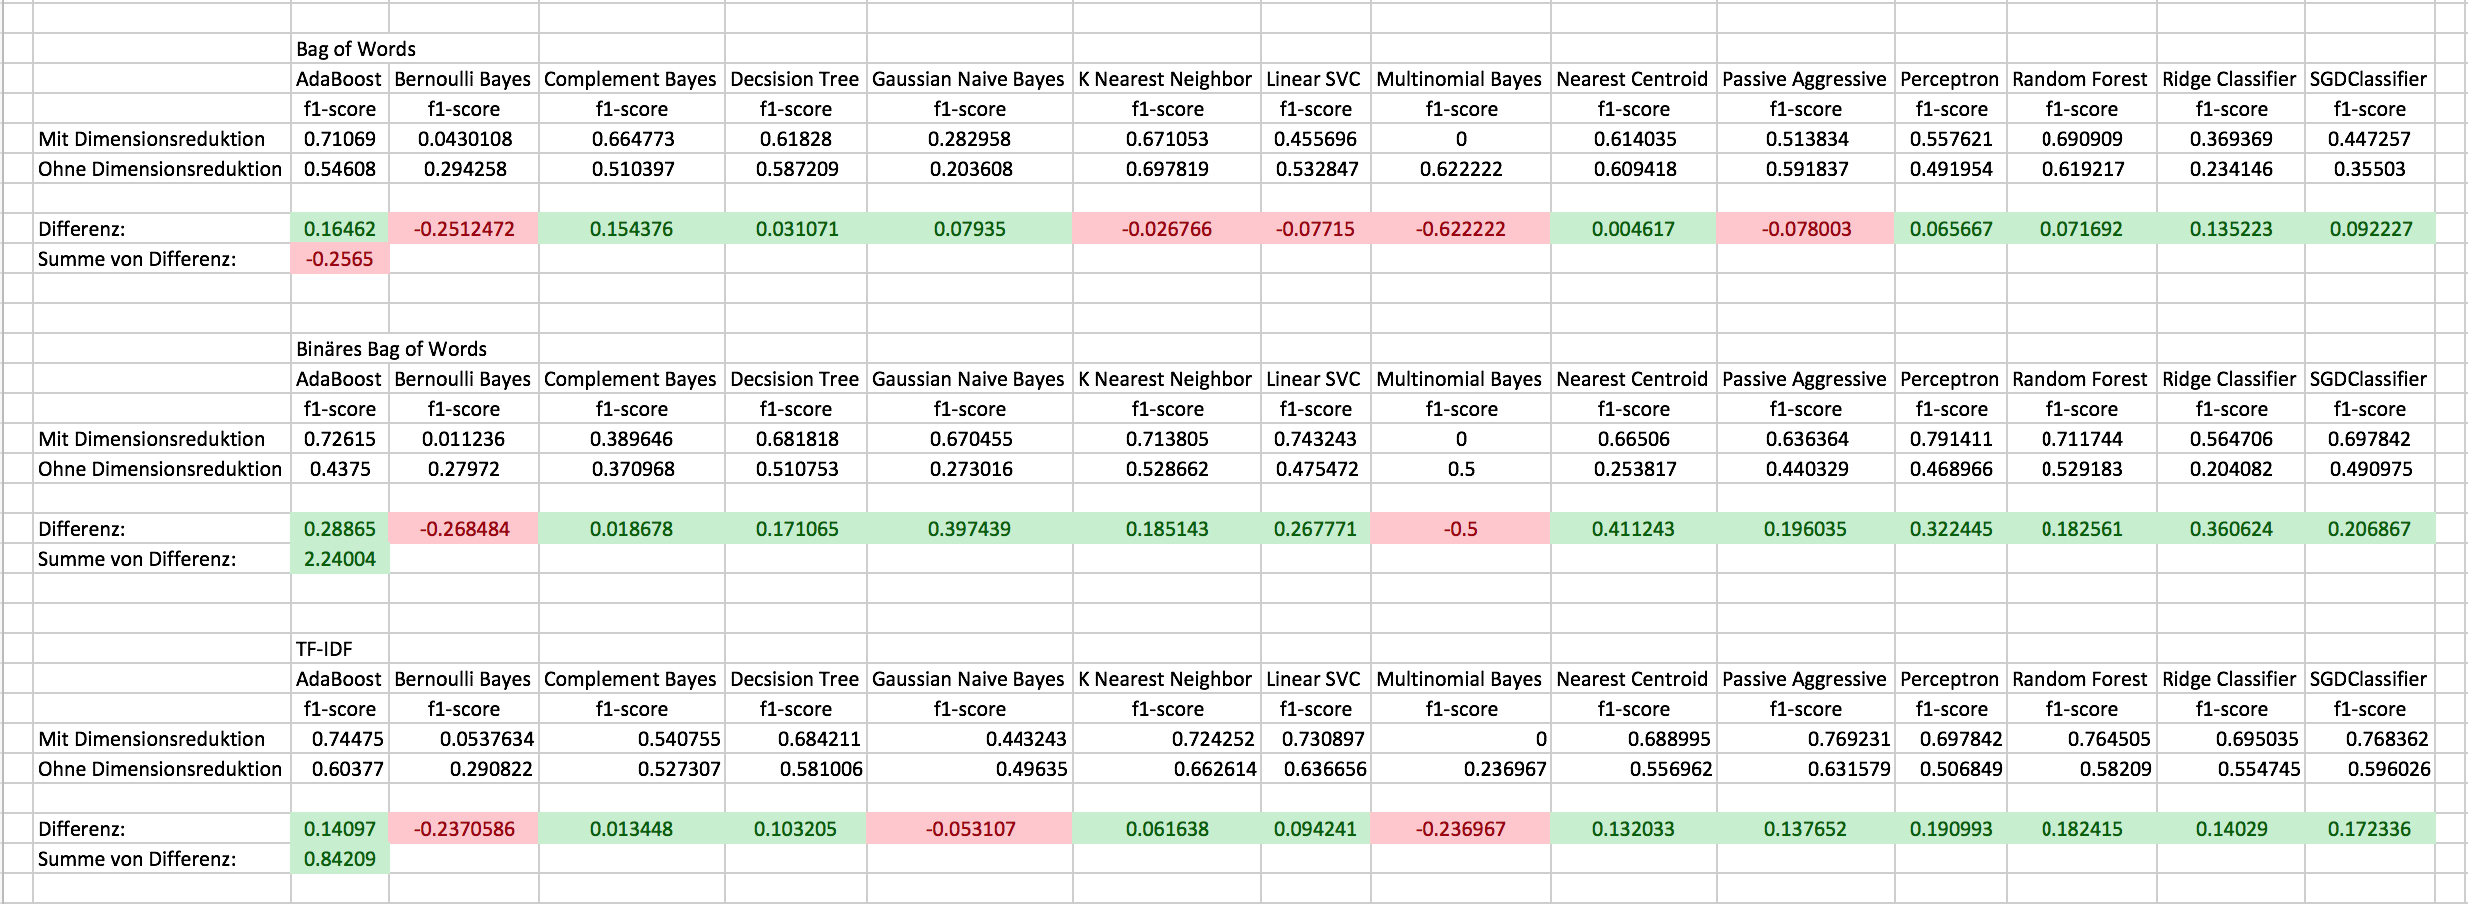
\includegraphics[width=1\columnwidth,keepaspectratio]{img/dimred.png}} 
	\caption{Grafik der Auswertung für die Dimensionsreduktion mittels LSA}
	\source{Eigene Darstellung}
	\label{abb:dimred}
\end{figure}
\subsection{Angabe von Klassenverteilung}
\subsubsection{Methoden}
Da die Daten aus dem Gold Standard eine sehr ungleiche Verteilung von positiven und negativen Samples aufweist, wurde die Klassengewichtung anhand dieser Verteilung berechnet.
Die Gewichtung, auf ein positives Sample folgen 10.32 negative Samples, wurde den Algorithmen fürs Trainieren mitgegeben.
Mittels der Klassenverteilung können die Algorithmen die unterrepräsentierten Klassen, in diesem Falle die positive Klasse, stärker gewichten und den Fokus darauf setzen.
Die Algorithmen wurden mit und ohne Klassengewichtung trainiert und validiert.
Zu erwähnen ist, dass die Gewichtung nicht allen Algorithmen zugewiesen werden konnte, da manche Algorithmen während dem Training solche Informationen nicht verwerten können.
\subsubsection{Resultate}
Die Angabe der Klassenverteilung konnte nicht bei allen Algorithmen als Parameter angegeben werden.
Somit werden alle Bayes-Algorithmen, KNearestNeighbor und Nearest-Centroid in der \cref{abb:classweight} nicht beachtet, da es dort zu keiner Veränderung der Scores kommt.\\
Bei beiden \glqq Bag of Words\grqq{} Methoden erzielt die Angabe der Klassenverteilung eine durchschnittliche Verbesserung der F1-Scores.
Einzelne Algorithmen reagieren negativ auf die Angabe, aber die positiven Auswirkungen übertreffen die negativen Auswirkungen.
Somit wird bei beiden \glqq Bag of Words\grqq{} Methoden die Angabe der Klassenverteilung miteinbezogen.\\
Bei der TF-IDF-Methode werden drei Algorithmen negativ und vier Algorithmen positiv beeinflusst.
Lediglich beim PassiveAgressiveClassifier gibt es eine markante Verschlechterung des F1-Scores.
Bei den anderen Algorithmen halten sich die negativen Auswirkungen im Rahmen.
Den F1-Score des PassiveAgressiveClassifier ausgenommen, sind die positiven Auswirkungen grösser als die negativen Auswirkungen.
Somit wird für TF-IDF ebenfalls die Angabe der Klassenverteilung für die nächsten Schritte beibehalten.
\begin{figure}[H]	
	\centering
	\setlength{\fboxsep}{0.3pt} 
	\setlength{\fboxrule}{0.3pt} 
	\fbox{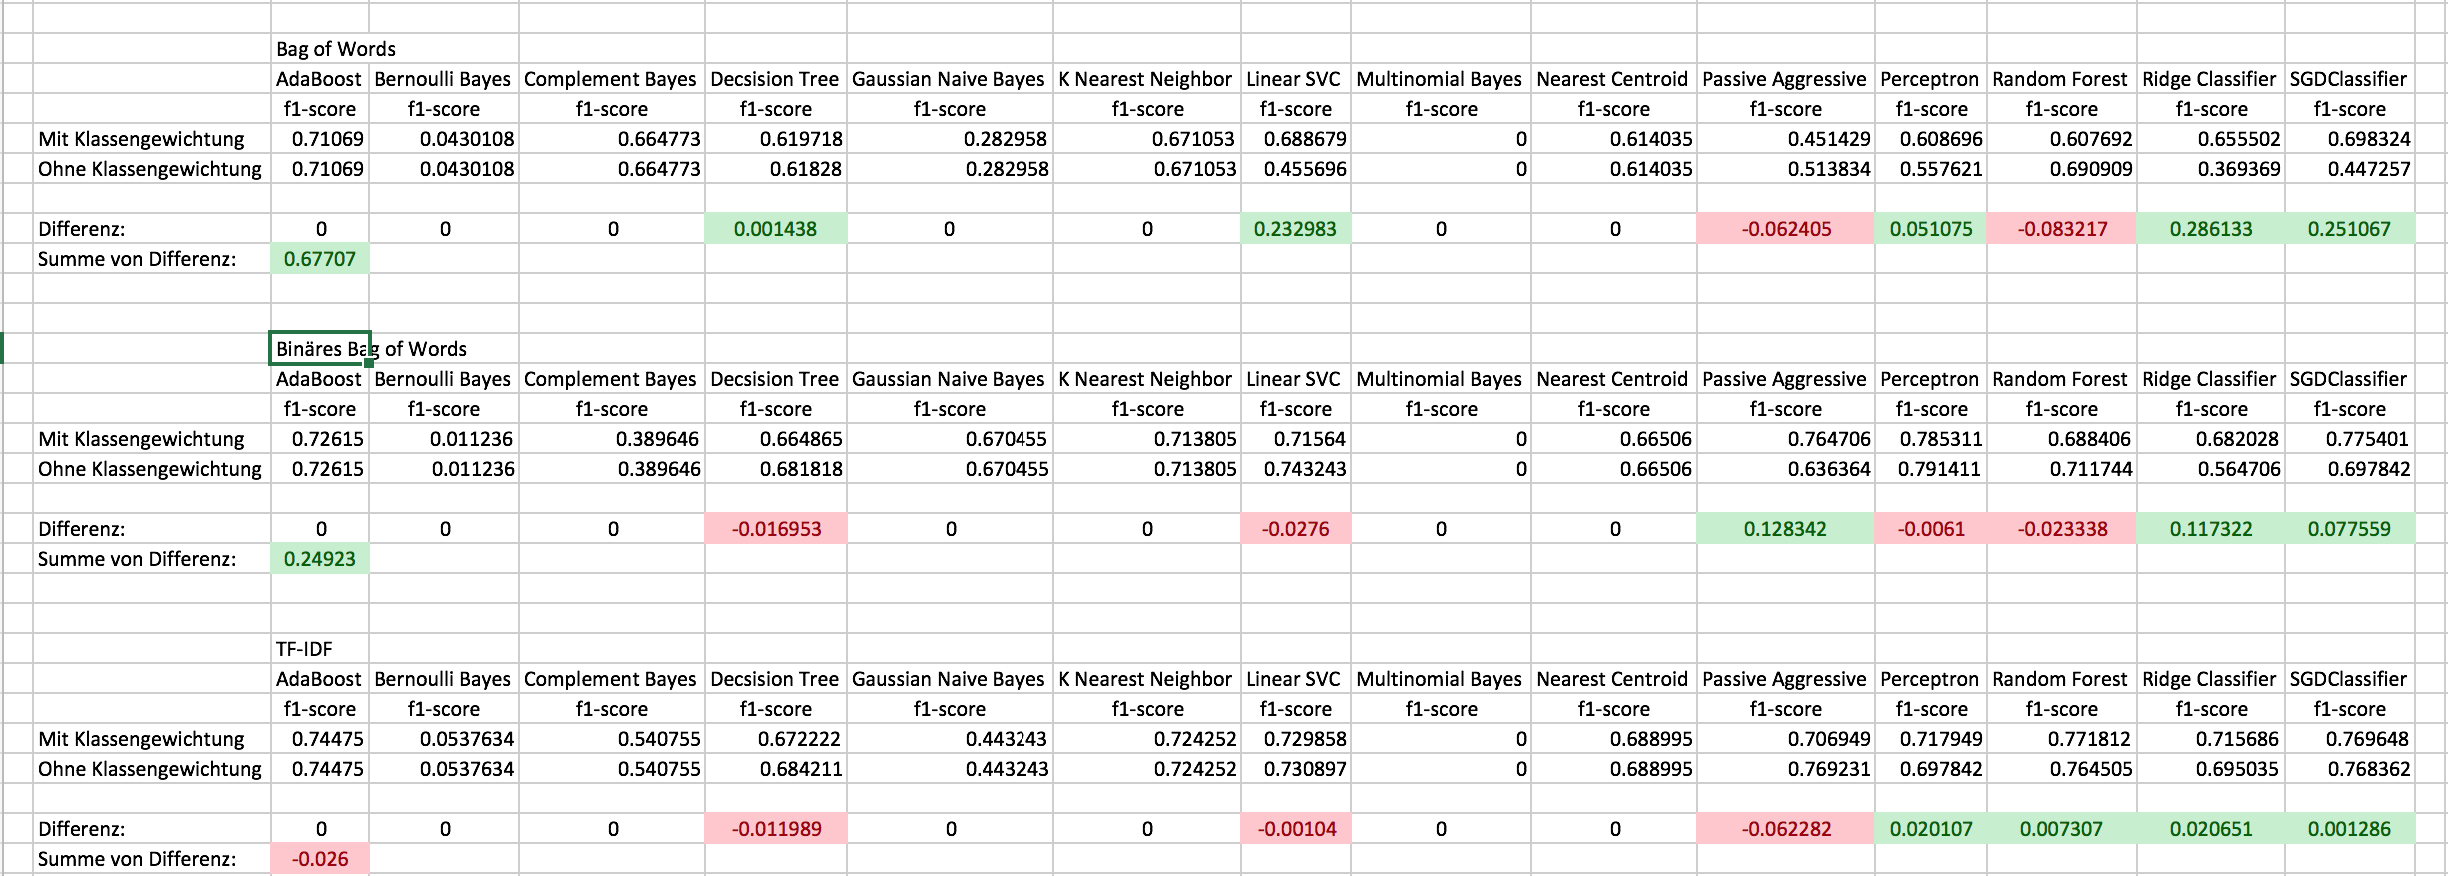
\includegraphics[width=1\columnwidth,keepaspectratio]{img/classweight.png}} 
	\caption{Grafik der Auswertung für die Klassenverteilung}
	\source{Eigene Darstellung}
	\label{abb:classweight}
\end{figure}
\subsection{Anwendung von N-Grammen}
\subsubsection{Methoden}
Die verwendeten Feature-Extraction Methoden bieten die Möglichkeit N-Gramme als Features zu extrahieren.
Aufgrund der Annahme der Autoren, dass verschiedene Menünamen oder Gerichtbezeichnungen in Form von Bi- oder Trigrammen auftreten (Cordon-Bleu, Prosciutto e Funghi), macht die Überprüfung von Bi- und Trigrammen Sinn.\\
Die Scikit-Learn Feature-Extraction Methoden bieten einfache Schnittstellen für die Extrahierung von N-Grammen.
Die Validierung von Uni-, Bi- und Trigrammen wurde für alle drei Feature-Extraction Methoden durchgeführt, die Algorithmen mit den neuen Features trainiert und wieder validiert.
\subsubsection{Resultate}
Die Ergebnisse sind in der \cref{abb:ngram} ersichtlich.
Bei beiden \glqq Bag of Words\grqq{} Methoden erzielt die Verwendung von Unigrammen die besten Ergebnisse.
Bi- und Trigramme können bei einzelnen Algorithmen ebenfalls eine Verbesserunge verzeichnen, aber im Vergleich zu Unigrammen fallen diese flächendeckend kleiner aus.
Somit werden bei beiden \glqq Bag of Words\grqq{} Varianten nur Unigramme verwendet.
Ebenfalls benötigt die Extrahierung der Features bei Bi- und Trigrammen etwa doppelt so lange, was eine enorme Performanceeinbusse ist.\\
Bei der TF-IDF-Methode erzielen Bi- und Trigramme die exakt gleichen Werte.
Dies ist zu erklären, da die TF-IDF Methode keine relevanten Trigramme gefunden hat und somit auf Bigramme zurückgegriffen hat.
Unigramme erzielen im Durchschnitt leicht bessere Werte im Vergleich zu Bi- und Trigrammen.
Jedoch sind von den fünf besten Ergebnissen drei mit Bi-, beziehungsweise Trigrammen erzielt worden, was anhand der gelb markierten Zellen ersichtlich ist.
Da die Entscheidung bei der TF-IDF Methode nicht eindeutig gefällt werden konnte, entschieden sich die Autoren für die Anwendung von Bigrammen.
\begin{figure}[H]	
	\centering
	\setlength{\fboxsep}{0.3pt} 
	\setlength{\fboxrule}{0.3pt} 
	\fbox{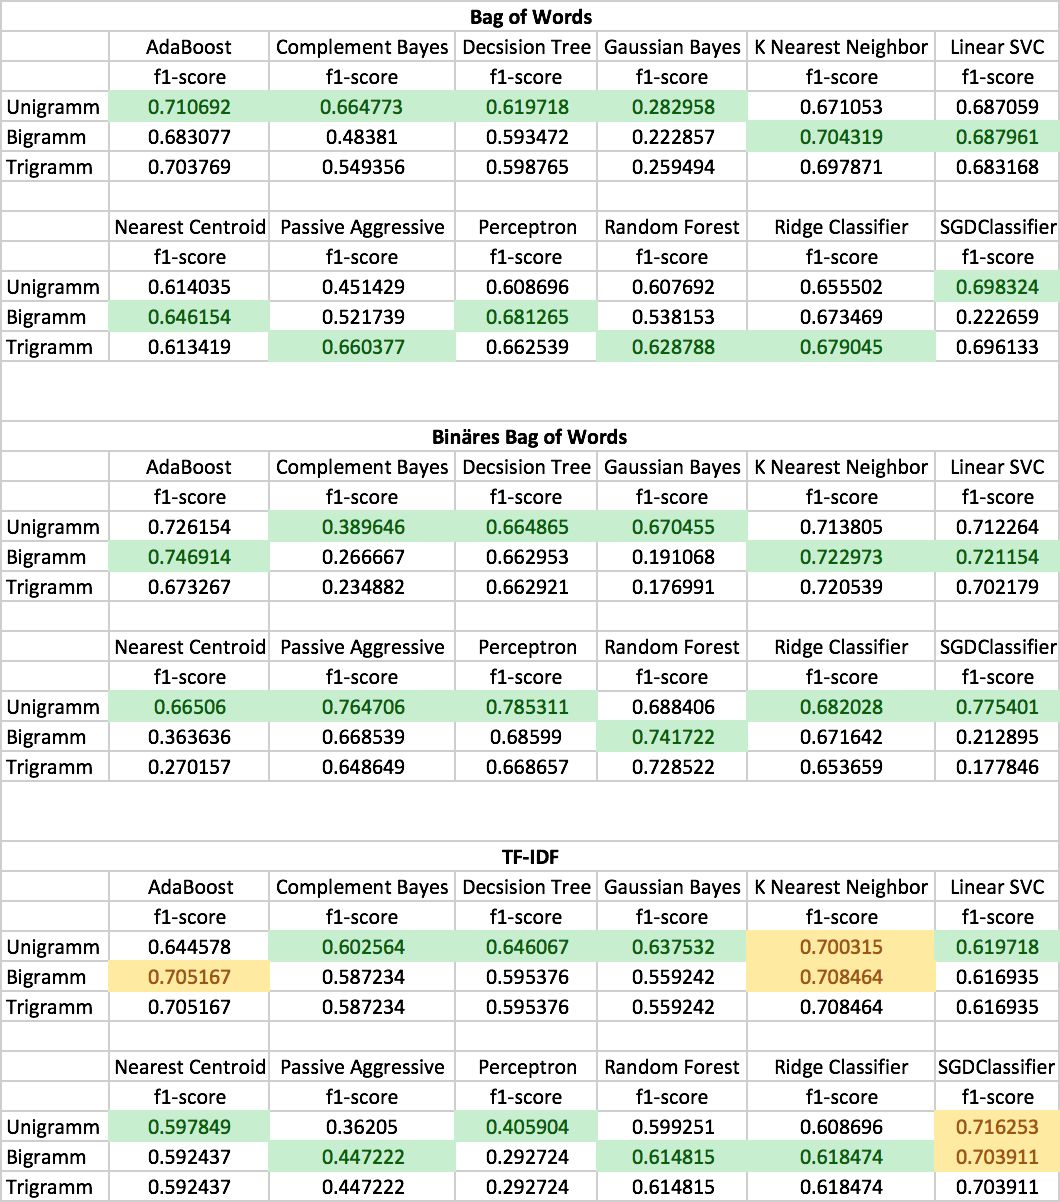
\includegraphics[width=1\columnwidth,keepaspectratio]{img/ngram.png}} 
	\caption{Auswertung der N-Gramme }
	\source{Eigene Darstellung}
	\label{abb:ngram}
\end{figure}
\subsection{Anwendung von fortgeschrittenen Preprocessingschritten}
\subsubsection{Methoden}
Fortgeschrittene Preprocessing-Schritte haben die Aufgabe den Text weiter zu modifizieren und die Extrahierung von zusätzlichen Informationen zu vereinfachen.
Im Kontext vom Machine-Learning Teil zählen folgende Preprocessingschritte zu den fortgeschrittenen Funktionen:
\begin{itemize}
	\item Das Markieren von Preisen mit entsprechenden Tags
	\item Die Stammformreduktion
	\item Das Entfernen von Stopwörtern
	\item Das Markieren von Information, die sich auf Getränke beziehen
\end{itemize}
Diese fortgeschrittenen Funktionen können ebenfalls im Unterkapitel \ref{sec:advancedpre} nachgelesen werden.
Es wurden die Auswirkungen von jeglichen Kombinationen der fortgeschrittenen Preprocessing-Schritten getestet.
Bei vier verschiedenen Arten ergeben sich 16 verschiedene Kombinationen.
\subsubsection{Resultate}
Das fortschrittliche Preprocessing erzielt bei allen drei Feature-Extraction Methoden keine eindeutigen Resultate.\\
Bei der \glqq Bag of Words\grqq{} Methode erreicht die Konfiguration \glqq config8\grqq{} mit dem Preisdetektor, der Stoppwörterentfernung und der Stammformreduktion die grössten positiven Einwirkungen.
Sieben Algorithmen können mit dieser Konfiguration ihre F1-Scores verbessern.
Somit wird für \glqq Bag of Words\grqq{} die Konfiguration \glqq config8\grqq{} weiter benutzt.\\
Bei der binären \glqq Bag of Words\grqq{} Methode gibt es bei keiner Konfiguration irgendwelche flächendeckenden Verbesserungen.
Es gibt jeweils nur vereinzelte Algorithmen, welche ihre Scores verbessern können.
Da keine Konfiguration eindeutig als Verbesserung angesehen werden kann, wird bei dieser Variante keine der fortgeschrittenen Preprocessing-Schritte angewendet.\\
Bei der TF-IDF-Methode gibt es ebenfalls keine eindeutigen Verbesserungen bei irgendeiner Konfiguration.
Es können vereinzelte Algorithmen ihre Scores verbessern, aber es findet nie flächendeckend eine Verbesserung statt.
Bei der Konfiguration \glqq config5\grqq{} erzielt AdaBoost den höchsten Wert über alle Konfigurationen gesehen, aber die anderen Algorithmen werden nur leicht beeinflusst.
Um bei der weiteren Ermittlung von Optimierungen nicht nur auf einen Algorithmus zu setzen, wird bei TF-IDF kein fortgeschrittenes Preprocessing angewendet.
\\\\
Die Auswertung für das fortschrittliche Preprocessing kann im Anhang \cref{app:electronic} im Zip-Ordner mit den Log- und Konfigurationsdateien gefunden werden.
\subsection{Anzahl Features}
\subsubsection{Methoden}
Jeder Algorithmus verhaltet sich mit der Änderung der Anzahl extrahierter und dimensionsreduzierter Features unterschiedlich.
Um eine optimale Anzahl an Features zu ermitteln, wurde die Anzahl Features schrittweise erhöht , die Algorithmen mit der neuen Anzahl trainiert und schlussendlich validiert.
Dies ist ein rechenintensives Unterfangen, führt in der Regel jedoch zu spürbaren Verbesserungen der Scores bei allen Algorithmen.
Die Messungen wurden mit einer Anzahl Features von 10 gestartet und schrittweise um 25 Features erhöht, bis schlussendlich eine maximale Anzahl von 400 Features erreicht wurde.
Da die Rechenzeit stetig mit der Erhöhung der Features steigt, wurde die Grenze bei 400 Features gesetzt.
Grundsätzlich macht eine Begrenzung der Features Sinn, da ab einer gewissen Anzahl Features die Algorithmen mit der Handhabung der Features überfordert sind und dies sich dementsprechend auf schlechteren Scores widerspiegelt.
\subsubsection{Resultate}
Für alle drei Feature-Extraction Methoden wurde ein Liniendiagramm für F1-Score, Precision und Recall erstellt.
Aus diesen Grafiken kann entnommen werden, bei welcher Feature-Anzahl welcher Algorithmus den besten Score erzielt.
Für die weitere Auswertung ist die Grafik für F1-Score massgebend und wird weiter analysiert.\\

\textbf{Bag of Words}\\
In der \cref{abb:bow-f1} ist ersichtlich, dass mit \glqq Bag of Words\grqq{} der Algorithmus AdaBoost bei 100 Features mit Abstand den besten F1-Score erzielt und fast die 0.8 Marke erreicht.
Ebenfalls kann der LinearSVC Algorithmus einen guten F1-Score erzielen und teilt sich mit AdaBoost die besten Werte.
Ersichtlich ist ebenfalls, dass die meisten Algorithmen sich zwischen 0.6 und 0.7 bewegen und das vereinzelte Klassifizierer mit ihren Werten auf und ab springen.\\
Die springenden Algorithmen Perceptron, SGDClassifier und PassiveAgressiveClassifier sind alle von der Familie \glqq Linear\_Model\grqq{}. Ein Grund für das auffällige Verhalten wurde nicht gefunden.
\begin{figure}[H]
	\centering	
	\setlength{\fboxsep}{0.3pt} 
	\setlength{\fboxrule}{0.3pt} 
	\fbox{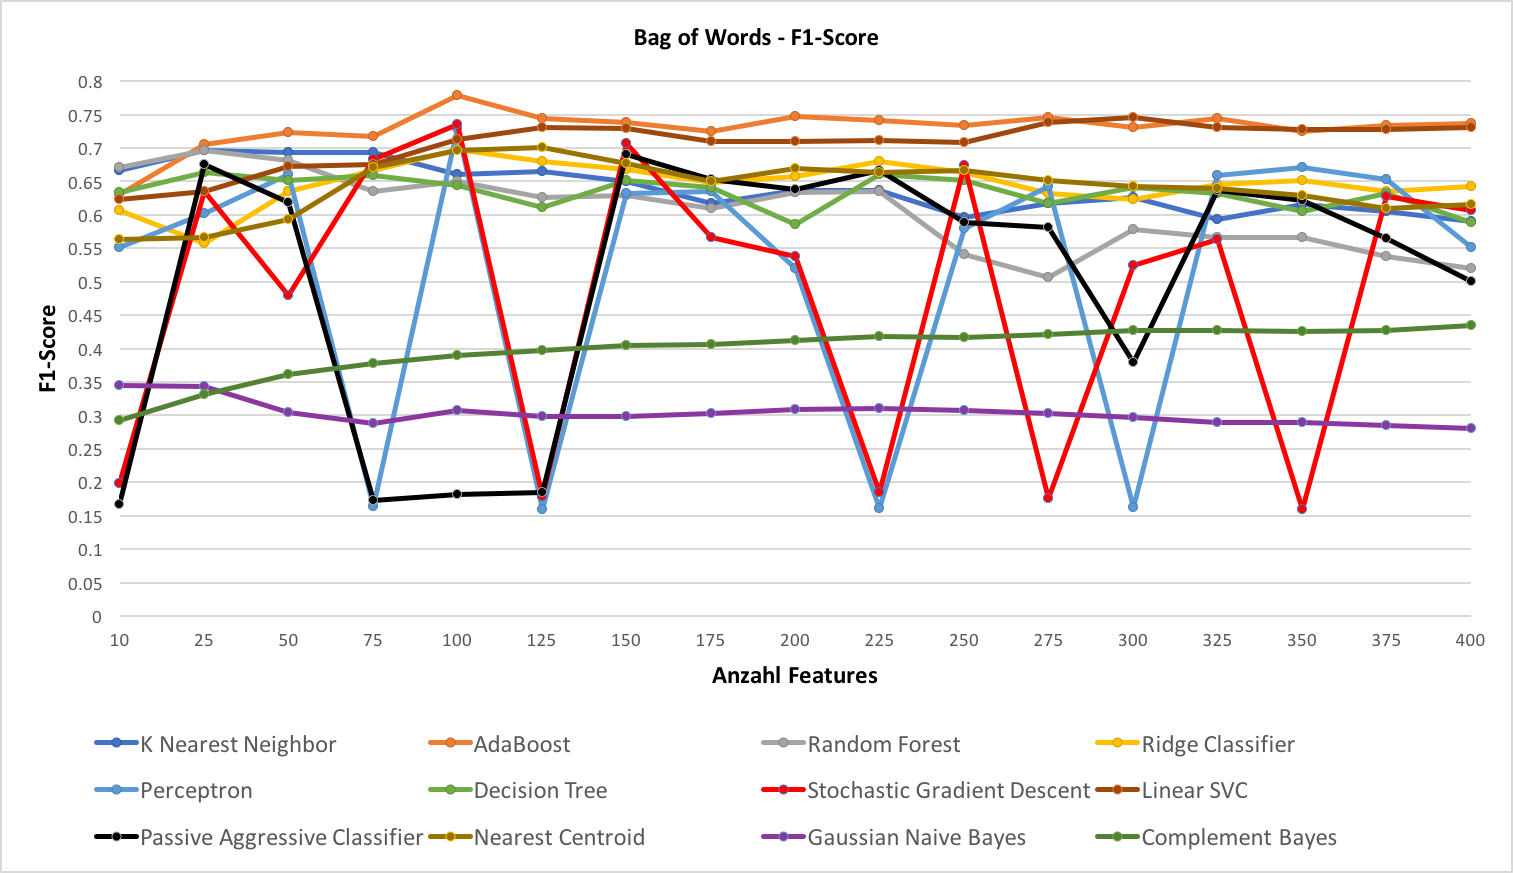
\includegraphics[width=1\columnwidth,keepaspectratio]{img/bow-f1.png}} 
	\caption{Grafik des F1-Score-Verlaufs bei Bag of Words}
	\source{Eigene Darstellung}
	\label{abb:bow-f1}
\end{figure}

\textbf{Binäres Bag of Words}\\
Bei der Methode \glqq binäres Bag of Words\grqq{} können mehrere Algorithmen einen F1-Score nahe der 0.8 Grenze verbuchen.
In der \cref{abb:bow-bin-f1} ist klar erkennbar, dass die meisten Algorithmen einen F1-Score zwischen 0.6 und 0.8 erzielen.
Der beste Algorithmus ist Perceptron, welcher mit 325 Features einen F1-Score von 0.8 verzeichnet.\\
Der SGDClassifier erreicht ebenfalls einen F1-Score von 0.8, jedoch mit einer höheren Anzahl von Features.
Dies bedeutet das SGDClassifier potenziell länger für die Feature-Extraction benötigt und somit ist Perceptron der favorisierende Algorithmus bei dieser Variante.\\
Die Sprünge der linearen Modelle, welche bereits bei der oberen \glqq Bag of Words\grqq{} Methode dargestellt wurden, sind ebenfalls wieder in der F1-Score-Grafik \cref{abb:bow-bin-f1} zu erkennen.
\begin{figure}[H]
	\centering	
	\setlength{\fboxsep}{0.3pt} 
	\setlength{\fboxrule}{0.3pt} 
	\fbox{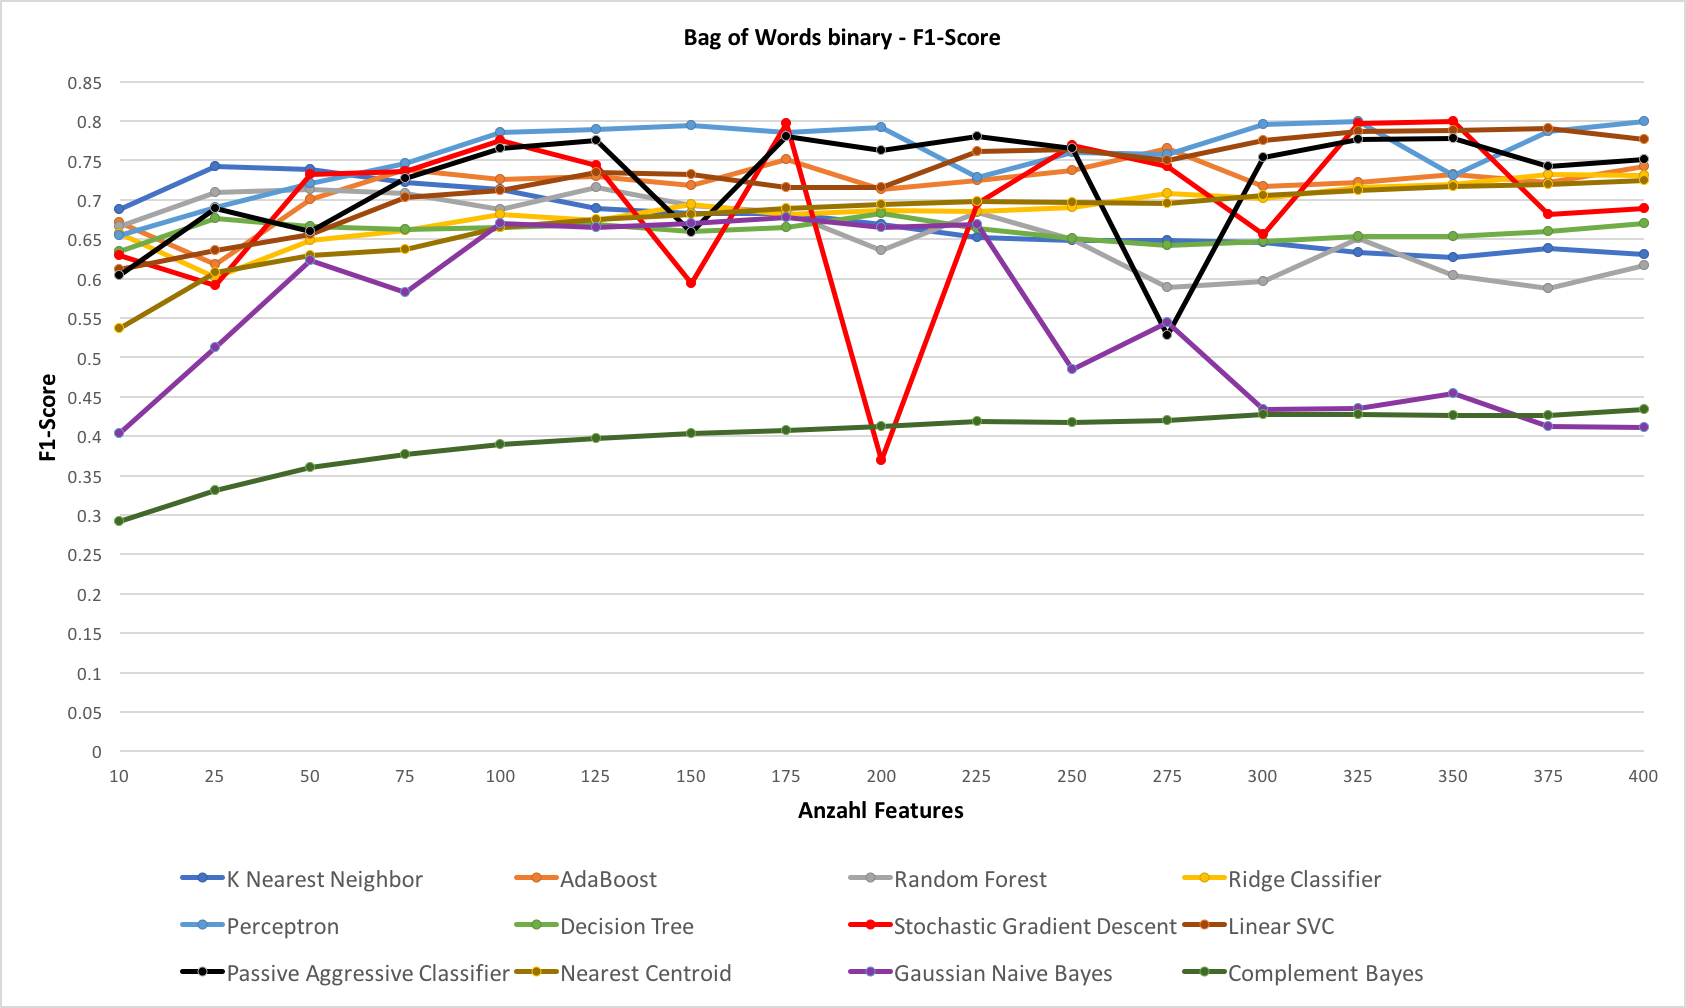
\includegraphics[width=1\columnwidth,keepaspectratio]{img/bow-bin-f1.png}} 
	\caption{Grafik des F1-Score-Verlaufs bei binärem Bag of Words}
	\source{Eigene Darstellung}
	\label{abb:bow-bin-f1}
\end{figure}

\textbf{TF-IDF}\\
Bei der Verwendung von TF-IDF sind mehrere Algorithmen mit ihren F1-Scores im Bereich 0.7 bis 0.8.
In der \cref{abb:tfidf-f1} ist erkennbar, dass der SGDClassifier Algorithmus als einziger die Grenze von 0.8 durchbrechen kann.
Dies erreicht er mit einer Anzahl Features von 150 und ist somit der Algorithmus mit dem besten F1-Score.\\
Auch bei der TF-IDF Methode sind wieder Sprünge bei den linearen Modellen in der F1-Score-Grafik \cref{abb:tfidf-f1} deutlich erkennbar.
\begin{figure}[H]	
	\centering
	\setlength{\fboxsep}{0.3pt} 
	\setlength{\fboxrule}{0.3pt} 
	\fbox{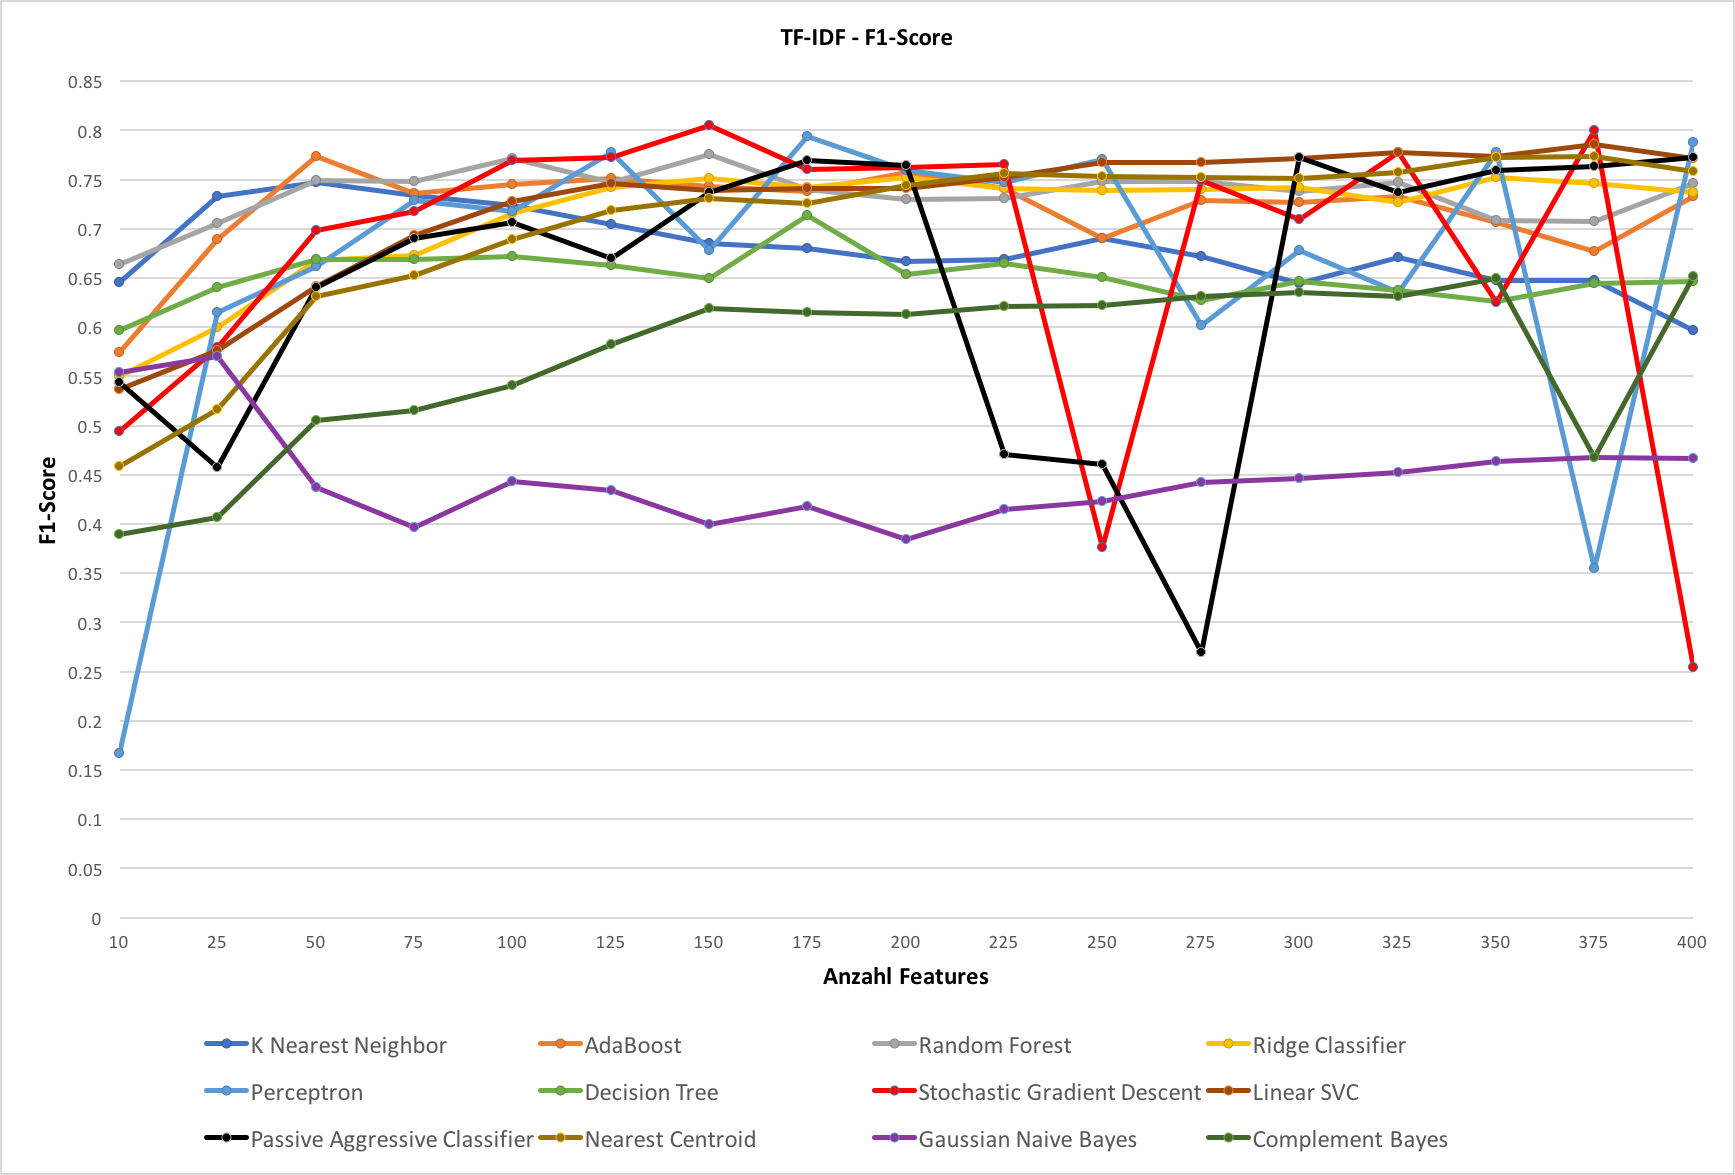
\includegraphics[width=1\columnwidth,keepaspectratio]{img/tfidf-f1.png}} 
	\caption{Grafik des F1-Score-Verlaufs bei TF-IDF}
	\source{Eigene Darstellung}
	\label{abb:tfidf-f1}
\end{figure}
\subsection{Hyperparametertuning}
\subsubsection{Methoden}
Als letzter Schritt der Algorithmenoptimierung wurde eine ausführliche Hyperparametersuche inklusive Kreuzvalidierung mit einem Wert von fünf durchgeführt.
Es wurden für die drei Feature-Extraction Methoden jeweils das Modell mit dem besten F1-Score kreuzvalidiert.
Für jedes Modell wurde eine Liste von anpassbaren Parametern zusammengestellt, welche Scikit-Learn vorgibt.
Für jeden Parameter wurde ein Bereich von möglichen Werten angegeben.
Mittels der Funktion \glqq GridSearchCV\grqq{}\footnote{\url{https://scikit-learn.org/stable/modules/generated/sklearn.model_selection.GridSearchCV.html}abgerufen am: 07.05.2019} von Scikit-Learn wurde die Hyperparametersuche für die Optimierung des F1-Scores durchgeführt.\\
Je nach Algorithmus und Grösse der Parameterliste kann die Hyperparametersuche sehr lange dauern.
Ebenfalls ist es möglich, dass die Standardparameter bereits ein Optimum darstellen und keine besseren Parameter gefunden werden.
\subsubsection{Resultate}
Die drei Modelle, welche aus dem vorherigen Experiment als die besten entnommen wurden, werden mittels Kreuzvalidierung auf optimale Hyperparameter durchsucht.\\
Die drei Modelle AdaBoost, SGDClassifier und Perceptron konnten die besten F1-Scores erzielen.\\
\begin{table}[H]
	
	\centering
	\label{tab:ada}
	\begin{tabular}{|l|l|l|l|}
		\hline
		& F1-Score & Precision & Recall\\
		\hline
		Vor Hyperparametertuning & 0.778 & 0.837 & 0.727 \\
		Nach Hyperparametertuning & 0.788 & 0.817 & 0.761 \\
		\hline
	\end{tabular}
	\caption{Auwertung Hyperparametertuning für AdaBoost mit binärem Bag of Words}
	\source{Eigene Darstellung}
\end{table}
\begin{table}[H]
	\centering
	\label{tab:per}
	\begin{tabular}{|l|l|l|l|}
		\hline
		& F1-Score & Precision & Recall\\
		\hline
		Vor Hyperparametertuning & 0.8 & 0.872 & 0.739 \\
		Nach Hyperparametertuning & 0.579 & 0.426 & 0.903 \\
		\hline
	\end{tabular}
	\caption{Auwertung Hyperparametertuning für Perceptron mit Bag of Words}
	\source{Eigene Darstellung}
\end{table}
\begin{table}[H]
	\centering
	\label{tab:sgd}
	\begin{tabular}{|l|l|l|l|}
		\hline
		& F1-Score & Precision & Recall\\
		\hline
		Vor Hyperparametertuning & 0.805 & 0.768 & 0.847 \\
		Nach Hyperparametertuning & 0.762 & 0.682 & 0.864 \\
		\hline
	\end{tabular}
	\caption{Auwertung Hyperparametertuning für SGDClassifier mit TF-IDF}
	\source{Eigene Darstellung}
\end{table}
In der \cref{tab:ada} ist auffällig, dass AdaBoost als einziges Modell bessere Hyperparameter mittels Hyperparametertuning finden konnte.\\
AdaBoost kann seinen Recall verbessern, gleichzeitig verschlechtert sich aber seine Precision.
Da die Recallsteigerung grösser als der Precisionabfall ist, wird der F1-Score nach oben korrigiert.\\
Die anderen beiden Modelle Perceptron in \cref{tab:per} und SGDClassifier in \cref{tab:sgd} erzielen mit den neuen Parametern schlechtere Werte.
Beide können den Recall verbessern, jedoch müssen sie massive Gefälle bei der Precision einbüssen.
Da die Precision viel stärker abgenommen, als der Recall zugenommen hat, wird der F1-Score schlechter.\\
Somit sind die Standardparameter für Perceptron und SGDClassifier für den \glqq Use-Case: Restaurant-Suchmaschine\grqq{} bereits optimal gewählt worden, da beim Hyperparametertuning eine ausführliche Liste von veränderbaren Parametern keine Verbesserung erzielen konnte.\\
Perceptron hat im Vergleich zum SGDClassifier einen leicht tieferen F1-Score, jedoch ist seine Precision deutlich höher.
Da für den schlussendlichen \glqq Use-Case\grqq{} Precision wichtig ist, wird das Perceptron-Modell für weitere Auswertungen verwendet.
Die Annahme der Autoren lautet, dass es bei einer Suchmaschine wichtiger ist, richtige Ergebnisse anstatt möglichst viele Ergebnisse zu finden.
Aufgrund dieser Annahme wird das Perceptron-Modell für eine produktive Pipeline weiterverwendet.

\section{Diskussion}
Die Resultate der Experimente der zwei verschiedenen Ansätze anhand der Testdaten zeigen, dass mit regelbasierten Methoden ein fast gleich guter Score erreichbar ist wie mit Machine-Learning.
Beide Ansätze erzielen eine hohe Precision.
Es ist jedoch zu berücksichtigen, dass die Resultate der regelbasierten Methode bei steigender Anzahl Daten schlechter werden.
Die zwei verschiedenen Ansätze werden nun genauer erläutert.
\subsection{Diskussion der Resultate der regelbasierten Experimente}
Der Regelsatz \glqq Menü im Titel\grqq{} hat im Bezug auf den F1-Score das schlechteste Ergebnis geliefert, dafür einen Precision-Wert von 1.
Es ist also keine Webpage fälschlicherweise als Menüseite klassifiziert worden.
Dafür wurden nur 16\% der Menüseiten erkannt.

Die Suche nach Preisen innerhalb des Textes hat ein besseres Ergebnis geliefert, 50\% der Menüseiten wurden als solche erkannt und zwei Webpages wurden fälschlicherweise als Menüseiten klassifiziert. 
Eine Kombination dieser beiden Methoden ergibt eine fast identische Klassifikation.
28 von 50 Menüseiten wurden erkannt, ebenfalls zwei wurden fälschlicherweise als Menüseiten klassifiziert.

Durch das Verwenden einer Blacklist und Whitelist wurden fast gleich viele Menüseiten korrekt erkannt. Bei 26, also ca. 52\% der erkannten Webseiten wurde nur eine Webpage als Menüseite klassifiziert, welche keine ist.

Die Klassifikation mit der Methode \glqq Bag of Words\grqq{} führt zu den besten Ergebnissen der regelbasierten Klassifikation.
31 von 50 Menüseiten wurden erkannt, zudem wurden 3 Webpages fälschlicherweise als Menüseiten klassifiziert.\\

Alle Methoden erreichten auf dem Testdatensatz eine hohe Precision, jedoch ist der Recall jeweils so tief, dass der F1-Score nicht die vorausgesetzte Marke von 0.8 überschreitet.
Alle Methoden der regelbasierten Klassifikation mit Ausnahme der Methode \glqq Bag of Words\grqq{} funktionieren unabhängig vom Trainingsdatensatz.
Beim Evaluieren der besten Konfigurationsparameter wurden diese auf einem Split des Trainingsdatensatzes (ein sogenanntes Validationsset) getestet.
Im Vergleich zu den Ergebnissen des Testsets ist bei allen Regeln zu erkennen, dass die Werte deutlich tiefer sind.
Daraus kann die Schlussfolgerung gezogen werden, dass mit einer steigenden Anzahl zu klassifizierenden Daten die Diversität dieser steigt, was sich negativ auf die Ergebnisse auswirkt.
Insgesamt ist zu erkennen, dass eine qualitativ und quantitativ hochwertige Klassifikation von Webpages mit einem regelbasierten Ansatz vor allem mit steigender Datendiversität nicht möglich ist.
In allen Fällen wurde eine erhebliche Anzahl der Menüseiten nicht gefunden.
Wenn man dies nun auf den Anwendungsfall einer Suchmaschine überträgt, werden viele Menüseiten nicht angezeigt.
Im Bezug auf die Resultate des Trainingsdatensatzes ist zudem die Precision markant gesunken.
Dadurch werden im Anwendungsfall viele Webpages angezeigt, welche keine Menüseiten sind.
\subsection{Diskussion der Experimente mittels Machine-Learning}
Bei allen Experimenten wurden die Modelle jeweils auf dem Validierungsset validiert.
Um nun die wirkliche Performance des besten Modells zu überprüfen, wird die Klassifizierung mit dem ungesehenen Testset durchgeführt.
Für die Auswertung werden der F1-Score, die Precision und der Recall aufgezeigt.
Zusätzlich wird eine Konfusionsmatrix erstellt, welche darlegt, wie viele Webpages korrekt oder falsch eingestuft worden sind.
\\\\
Hinweis: Beim Perceptron wurde bei der Hyperparametersuche keine besseren Parameter gefunden.
Aufgrund dessen wurden die Standardparameter weiter verwendet.

\begin{table}[H]
	\centering
	\label{tab:bestclf}
	\begin{tabular}{|l|l|l|l|}
		\hline
		Methode & F1-Score & Precision & Recall\\
		\hline
		Perceptron mit binärem Bag of Words & 0.78 & 0.92 & 0.68 \\
		\hline
	\end{tabular}
	\caption{Bester Algorithmus der Machine-Learning Klassifikation}
	\source{Eigene Darstellung}
\end{table}

\begin{table}[H]
	
	\centering
	\label{tab:conf}
	\begin{tabular}{@{}cc|cc@{}}
		\multicolumn{1}{c}{} &\multicolumn{1}{c}{} &\multicolumn{2}{c}{Predicted} \\ 
		\multicolumn{1}{c}{} & 
		\multicolumn{1}{c|}{} & 
		\multicolumn{1}{c}{Positiv} & 
		\multicolumn{1}{c}{Negativ} \\ 
		\cline{2-4}
		\multirow[c]{2}{*}{\rotatebox[origin=tr]{90}{Actual}}
		& Positiv  & 34   & 16   \\[1.5ex]
		& Negativ  & 3   & 47 \\ 
		\cline{2-4}
	\end{tabular}
	\caption{Konfusionsmatrix der Methode: Perceptron mit binärem Bag of Words}
	\source{Eigene Darstellung}
\end{table}
In der \cref{tab:bestclf} ist ersichtlich, dass im Vergleich zur \cref{tab:per} der F1-Score leicht abgenommen hat.
Dies hat den Grund, dass der Recall spürbar an Wert verloren hat.
Die Precision jedoch stieg und wirkte der Reduzierung des F1-Scores entgegen.\\
In der Konfusionsmatrix (\cref{tab:conf}) ist deutlich die hohe Precision zu erkennen.
Der Algorithmus klassifizierte 34 Webpages korrekt als Menüseiten.
Ebenfalls wurden nur drei Webpages als Menüseiten klassifiziert, welche aber keine gewesen sind.
Die schlussendliche Performance des Klassifizierers ist für den genannten \glqq Use-Case\grqq{} zufriedenstellend und somit wird der Algorithmus Perceptron in einer produktiven Pipeline weiterverwendet.
\\\\
Schlussendlich ist ersichtlich, dass die Variante mit dem Perceptron-Algorithmus eine qualitative und quantitative Klassifizierung von Menüseiten erzielen kann.
Der F1-Score liegt zwar leicht unter dem selbst definierten Schwellwert von 0.8, jedoch ist die Precision mit 0.92 weit darüber.\\

Für den Anwendungsfall einer Suchmaschine ist es besser, wenn nicht möglichst viel gefunden wird, sondern dass das Gefundene effektiv korrekt ist.
Dennoch dürfen nicht nur eine Hand voll Menüseiten gefunden werden, damit das Angebot nicht verkümmert.\\
Der Perceptron-Algorithmus bietet einen guten Kompromiss zwischen Precision und Recall und wird deshalb für die Suchmaschine verwendet.
Mit seiner Precision von 0.92 erreicht er bei 37 Vorhersagen nur drei falsche Einschätzungen.
Somit wäre in der Suchmaschine jeder 13. Vorschlag falsch, was nach der Meinung der Autoren vertretbar ist.
\section{Beantwortung der Forschungsfrage}
Unter Verwendung der Daten des selbst erarbeiteten Gold Standards und dem selbst vorgegebenen Ziel eines F1-Scores von mindestens 0.8 lautet die Antwort auf die Forschungsfrage:\\

\emph{Nein, Restaurant-Webseiten können mit den erarbeiteten Klassifizierern nicht mit hoher Wahrscheinlichkeit klassifiziert werden, ob sie Menüinformationen beinhalten.}\\

Jedoch ist der angestrebte Wert auf den Testdaten nur knapp verfehlt worden, auf den Trainingsdaten wurde er sogar erreicht.
Es lässt sich vermuten, dass mit Anpassungen an den Algorithmen sowie der Daten das Ziel erreichen lässt.
Gründe für das Verfehlen des Ziels und Massnahmen, um dieses trotzdem noch zu erreichen, sind in \cref{chap:fazit} zu finden.


